\chapter{Experiment}
\label{chap:experiment}

A Time Projection Chamber (TPC) is a detector that reconstructs the energy loss of charged particles and the location of that energy loss as in all 3 dimensions within the detector. TPCs have been employed in gases, liquid, and even solid detectors \cite{starTPC,arTPC,eosTPC}. In the following, we outline the physical principles involved in measurements within a gaseous TPC, and discuss the particular details of the TPC used in this Thesis, along with the rest of the experimental setup.


\section{Operational Principles of Time Projection Chambers}

%explain in breif the basics of a time projection chamber 
\begin{figure}[!htb]
\centering
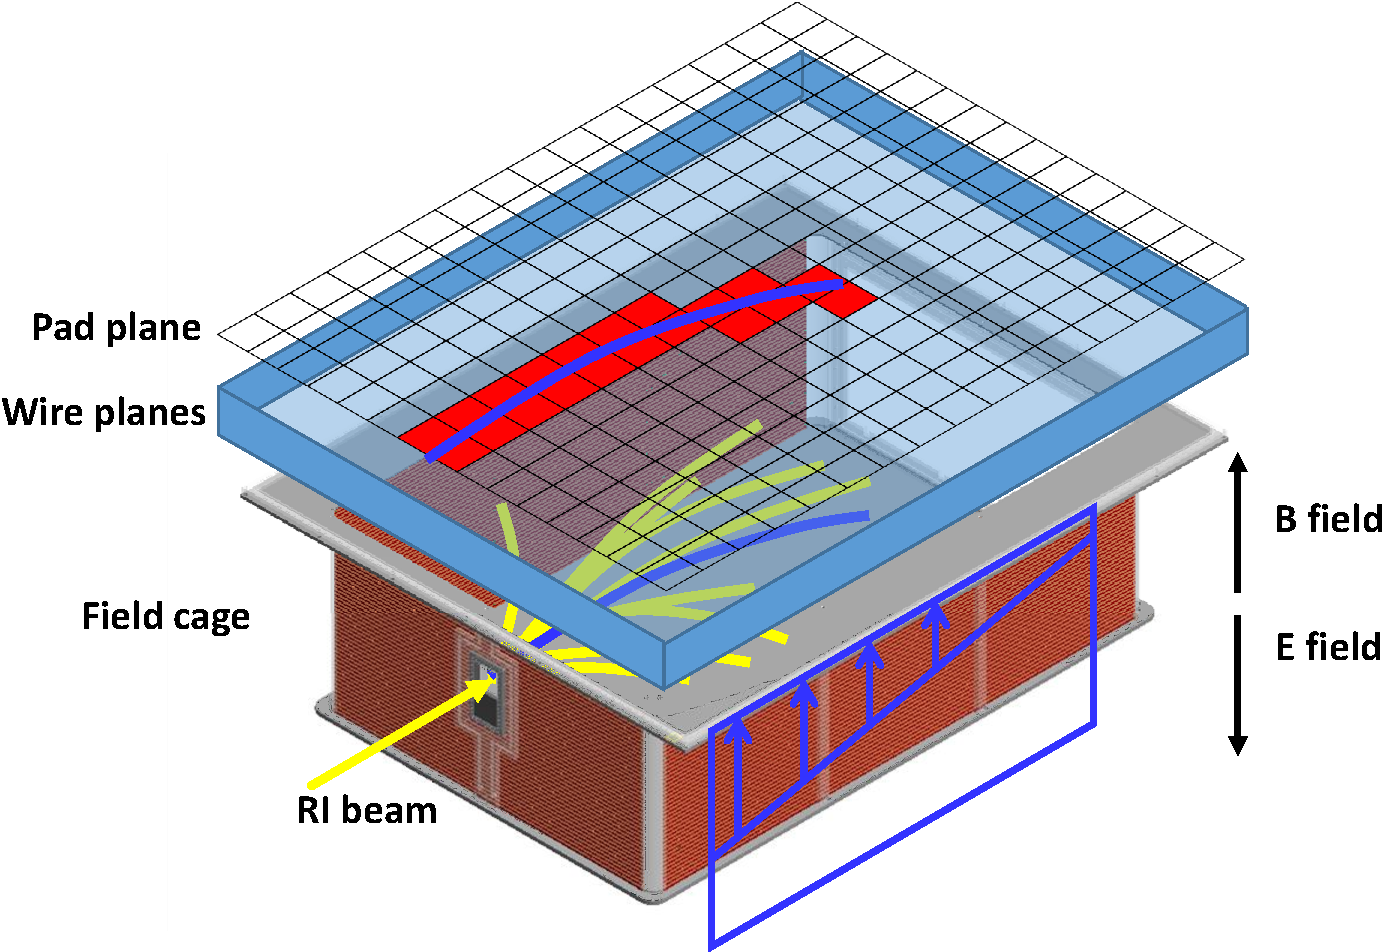
\includegraphics[scale=.5]{tpcPrinciple.pdf}
\caption{Cartoon depicting the operating principles of the TPC is.}
\label{fig:tpcPrinciple}
\end{figure}

%explain in breif the basics of a time projection chamber 
Figure~\ref{fig:tpcPrinciple} depicts the interior of a gaseous TPC and its field cage. The field cage holds the detector gas and also defines a constant electric field that is typically aligned with the magnetic field of a magnet that surrounds the TPC. In this Spirit TPC, both these electric and magnetic fields are vertical.  

As a charged particle resulting from a heavy ion collision passes through the field cage, energetic \emph{primary} electrons are knocked out of neutral gas molecules and atoms in the detector gas. These primary electrons further ionize the detector gas until there is a distribution of \emph{secondary} electrons and positive ions that lie along the track's path. The electric field of the field cage separates these electrons and ions, where the electrons are accelerated upward by the electric field in the direction against the electric field, and the positive ions are accelerated along the electric field. Since the mean free path of the electrons inside the gas is very small, they quickly collide with other gas molecules, which slow down, or even stop the electron; only to be re-accelerated by the electric field, continuing a repeating cycle of stop and go motion. This microscopic behavior results in a constant drift velocity when averaged over multiple gas collisions. 

The electrons drift with this drift velocity through a set of wire planes, eventually reaching a set of high voltage anode wires, where they quickly accelerate in the presence of the high electric field emanating from the anode wires. This high electric field imparts enough energy between collisions to ionize the gas, creating additional electron-ion pairs from the gas, culminating in an avalanche process near the anode wires. The avalanche electrons typically terminate on the anode wire,  while the ions created in the avalanche are accelerated  away from the anode wires. This ionic motion induces image charges in nearby pads within the pad plane that is located close to the anode wires. The corresponding image currents in these pads are read out by electronics that are attached to these pads. This electronics signal encodes the energy loss information and arrival time of the signal from the electrons drifting from the ion track, and can be analyzed to determine the position of the ion track within the TPC. 

The pad plane is perpendicular to the electric field of the field cage and is divided into a two dimensional grid of pads. Two of the 3 coordinates are determined from the 2-dimensional charge distribution corresponding to the projection of the track onto the pad-plane. The third dimension comes from extrapolating the electrons back in time, utilizing the known constant drift velocity $v_d$. The distance the electron has traveled , $d$, -- along the electric field direction-- is calculated as $d = v_d \cdot t$, where $t$ is the drift time information obtained from combining the time of the event trigger with arrival time of the signal from the  electrons in the electronics. The radius of curvature of the track on the pad plane is related to the magnetic rigidity, and therefore the momentum of each track. The energy loss deposited $\langle dE/dx\rangle$ is proportional to the image charge induced on the pads on the pad-plane. With these two observations, particles can be uniquely identified by their mass and charge since there is a unique correlation between the rigidity and $\langle dE/dx\rangle$  lines. This correlation allows the particle type to be identified as discussed later in Section~\ref{sec:pid}. In this chapter we will provide more details about the particle detection within the \spirit TPC  that is relevant to the reactions studied in this thesis. 


\section{S$\pi$RIT TPC Overview}
%Add Overview image with labels

\begin{figure}[!htb]
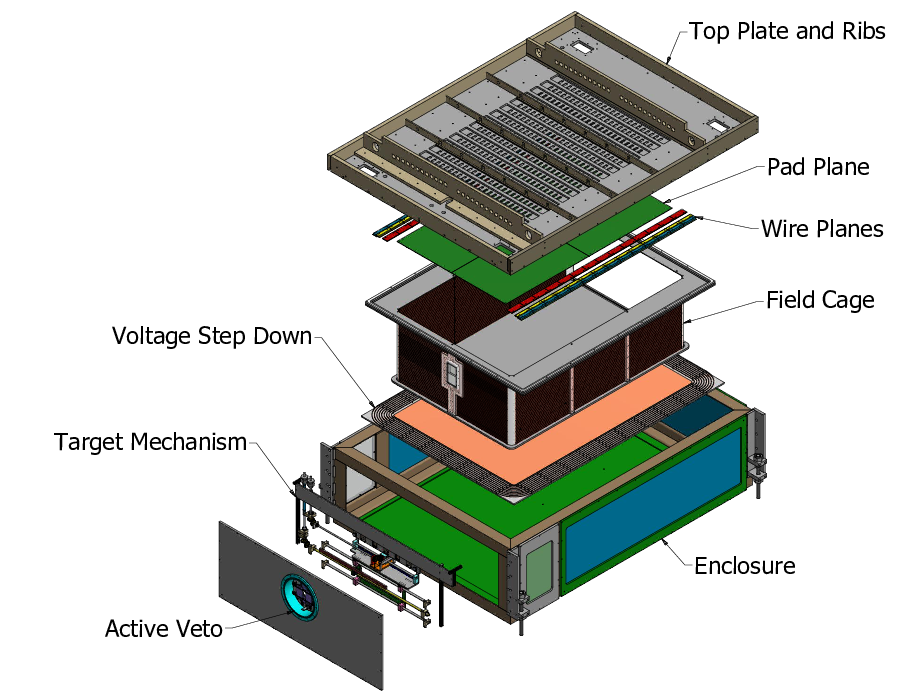
\includegraphics[width=\textwidth]{exploded.png}
\caption{Exploded overview of the of the \spirit TPC}
\label{fig:tpcExplode}
\end{figure}


The Samurai Pion-Reconstruction and Ion Tracker Time Projection Chamber (\spirit TPC) was developed to measure pions and other light charge particles produced in collisions of radioactive rare isotope beams with stable targets in fixed target experiments.  The TPC is built on an aluminum angle iron skeleton with thin aluminum sheet walls in order to minimize neutron scattering and to allow for light charged particles to reach auxilliary detectors on the sides and downstream of the TPC. The \spirit TPC was developed to fit inside the SAMURAI dipole magnet used at the Rare Isotope Beam Factory (RIBF) at RIKEN in Wako-shi, Japan \cite{riken}. The dipole gap limited the vertical space of the TPC to around \SI{75}{\centi\metre}. More detail and specifications of the SAMURAI dipole magnet are given in \cite{samurai}. 

The exploded drawing shown in Fig.~\ref{fig:tpcExplode} illustrates these major internal components of the  of the \spirit TPC. A target mechanism allowed for up to 5 fixed targets to be mounted on the target ladder situated just upstream of the field cage, where changing the targets could be performed outside of the magnet. Reaction products from nuclear collisions exit the target and enter the field cage of the TPC. The field cage contains the detector gas and defines the constant electric field. It is rigidly mounted to the large aluminum top plate of the TPC gas containent vessel. The field cage is electrically isolated from the top plate by a lexan top perimeter ring with o-rings to provide as gas seal. The pad plane and wire plane structures are  mounted to the inside face of the top plate with the electronics being mounted on the outside face of the top plate. Several aluminum ribs were also mounted to provide extra rigidity to the top plate, keeping it flat to within \SI{150}{\micro\metre}, as measured by a precise laser measurement \cite{jon}. Holes in the top plate allowed signals from the individual charge sensitive pads on the pad plane to be transmitted via cables to the electronics. 



\begin{table*}\centering
\ra{1.3}
\begin{tabular}{@{}rr@{}}\toprule 
\multicolumn{2}{c}{\spirit TPC Overview} \\
 \midrule
Pad plane area & 1.3 m x .9 m\\
Pad size       & 1.2 cm x .8 cm \\
Number of pads & 12096 (112 x 108) \\
Gas composition& 90\% Ar + 10\% CH${}_4$ (1 atm)  \\
Multiplicity limit & 200  \\
dE/dx range        & Z=1-3, $\pi$, p, d, t, He, Li \\
Drift length       & 50 cm \\
\bottomrule
\end{tabular}
\caption{Summary of general properties of the \spirit TPC.}
\label{tb:spiritoverview}
\end{table*}


\begin{comment}
\subsection{Enclosure}
The skeleton of the enclosure is composed of a rigid rectangular aluminum angle-iron frame. To this frame, six rectangular sides are attached. The downstream window and the two side windows are constructed of a aluminum window frames with a 1 mm  aluminum sheet metal window. These thin sheet metal windows allow charged particles and neutrons to exit the TPC without significant energy loss or scattering. This allows for a trigger to be created by placing detectors outside of  the side windows and downstream window of the TPC. The enclosure itself is made to be gas tight with no leakage from the outside or from the interior of the field cage. This is to allow for the possibility to choosing one insulation gas outside of the field cage and a different counter gas inside the field cage. In the first campaign of experiments, however, we used the same gas in the field cage and enclosure volume.  
\end{comment}

\subsection{Field Cage}
%The field cage contains the detector gas and defines a uniform electric field in which electrons can drift upwards toward the anode wires. It was designed to hang from the top plate and therefore needed to be of a lightweight construction and the materials needed to be thin to allow for light charged particle and neutrons to pass through to ancillary trigger detectors without significant energy loss or scattering .  

\begin{figure}[!htb]
\centering
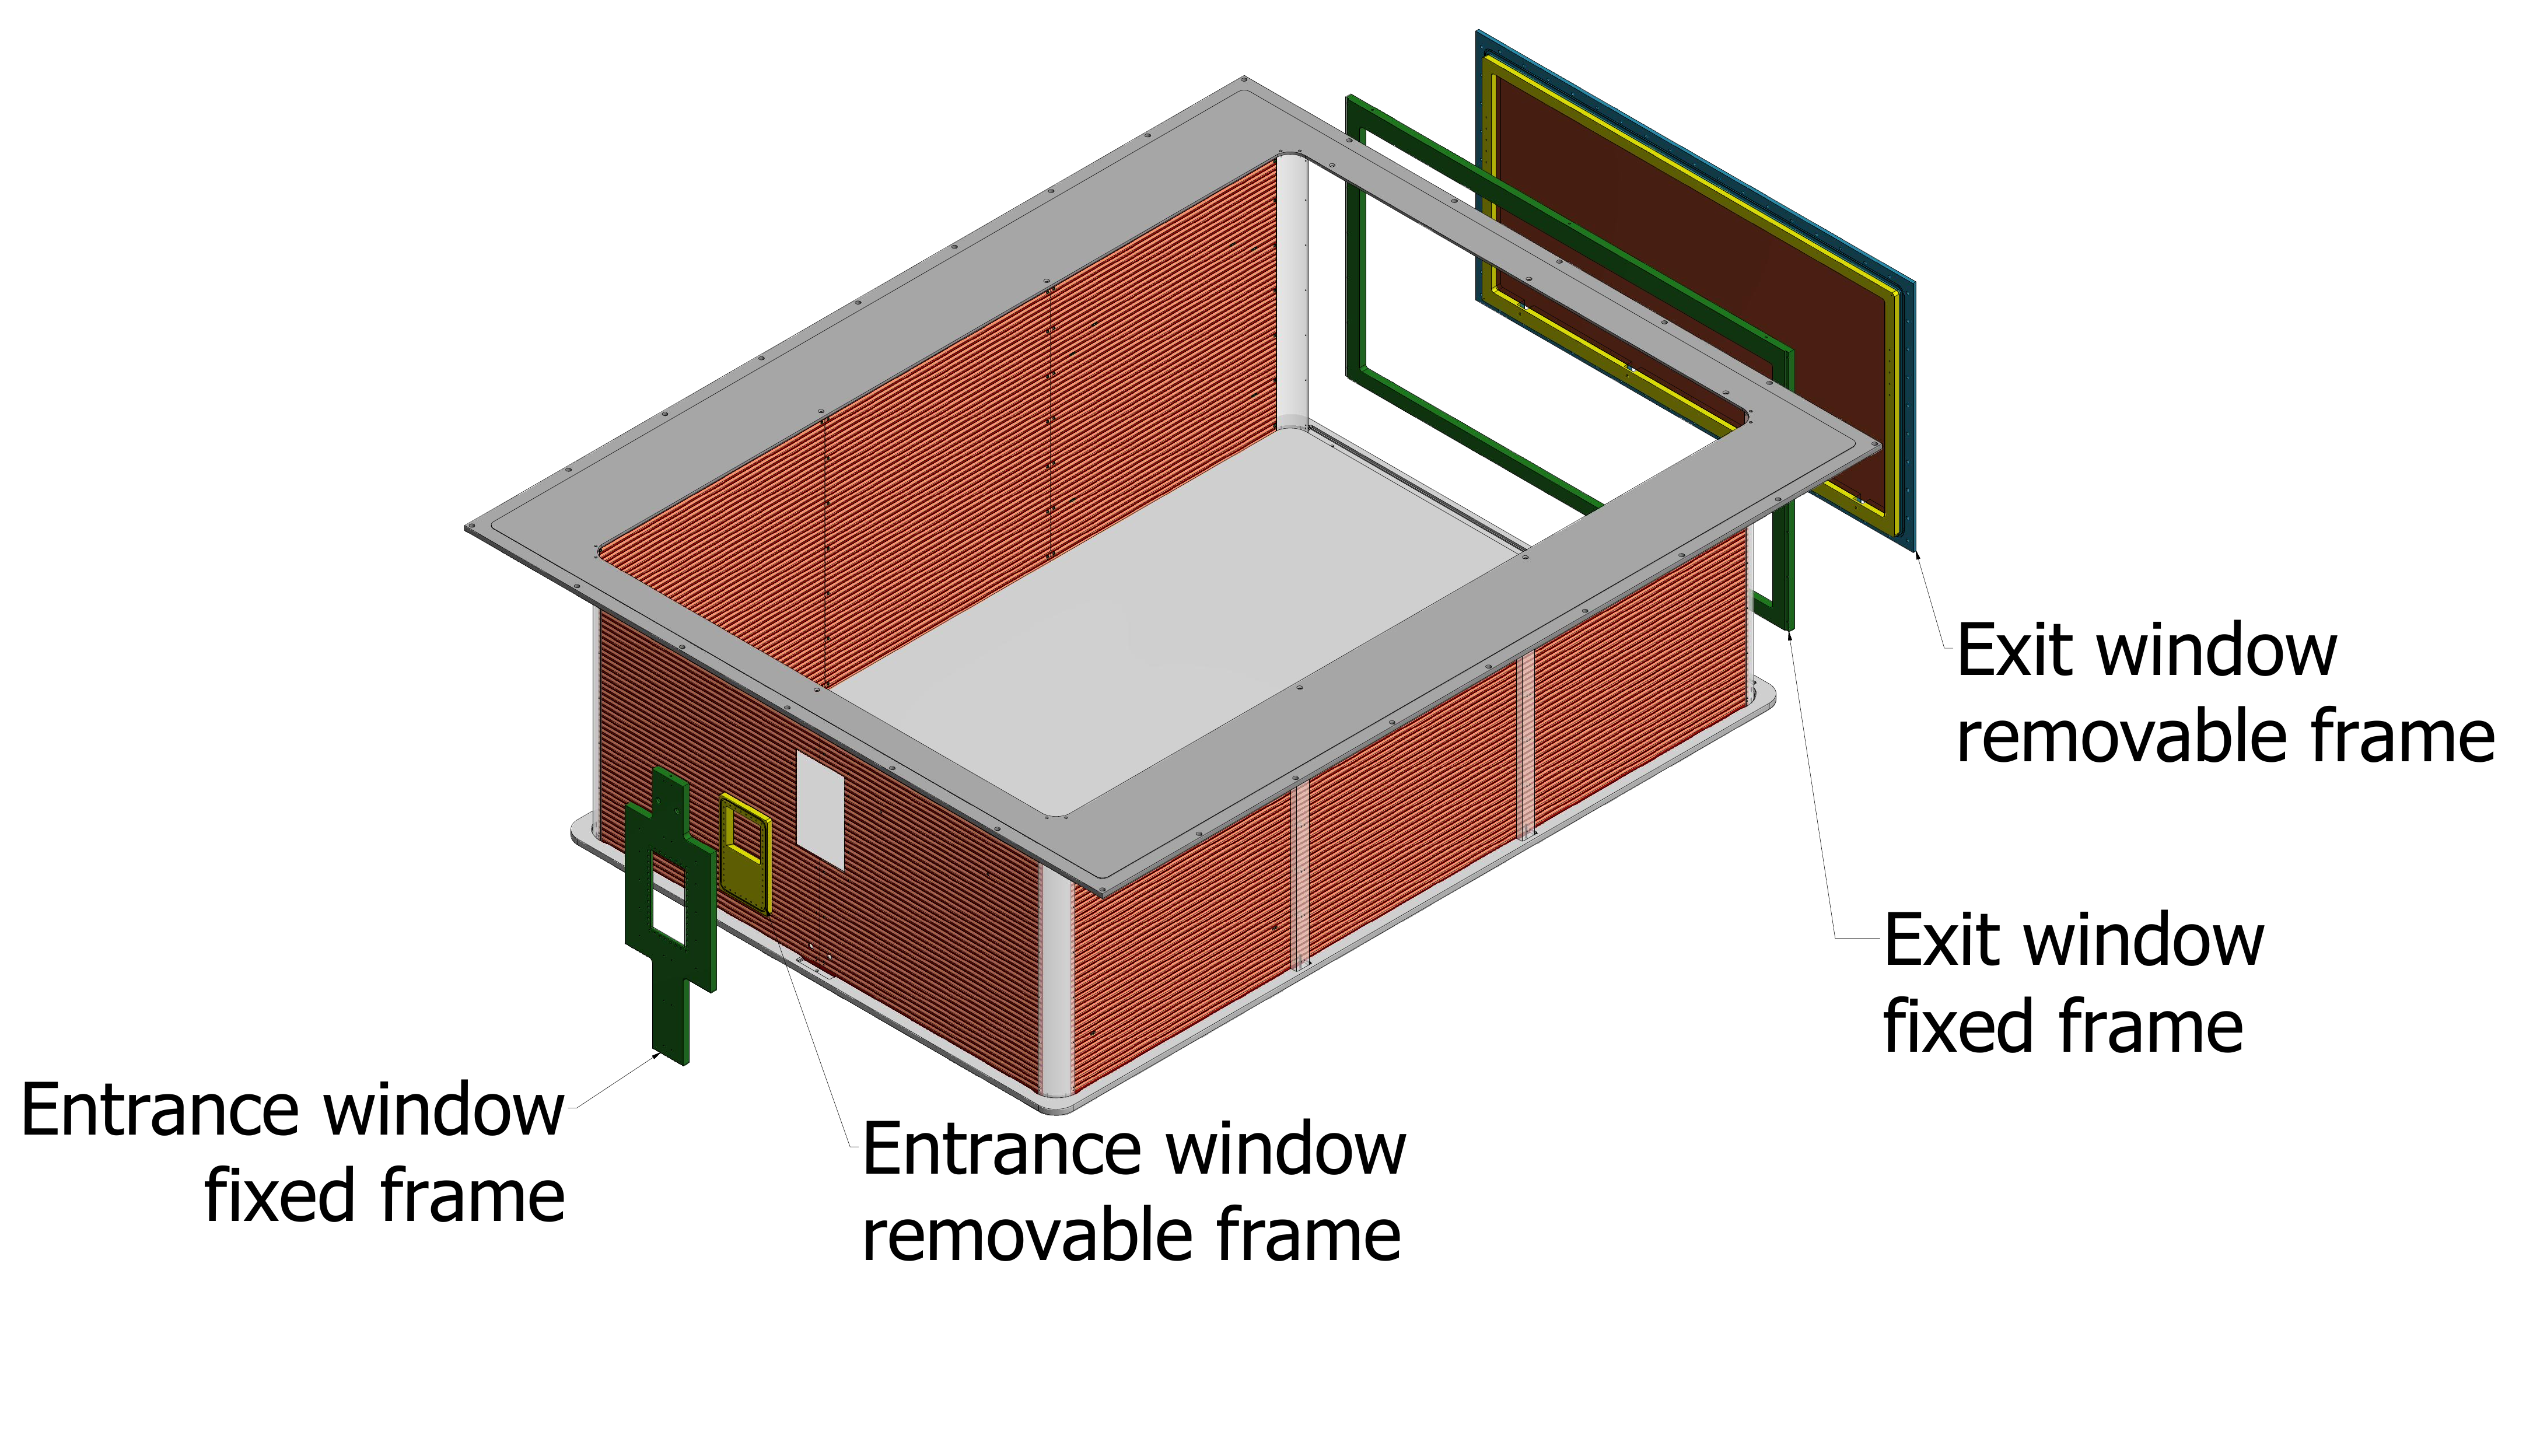
\includegraphics[width=.9\textwidth]{fc_overview.png}
\label{fig:fc_overview}
\caption{Overview of the field cage mechanical components.}
\end{figure}


\begin{figure}[!htb]
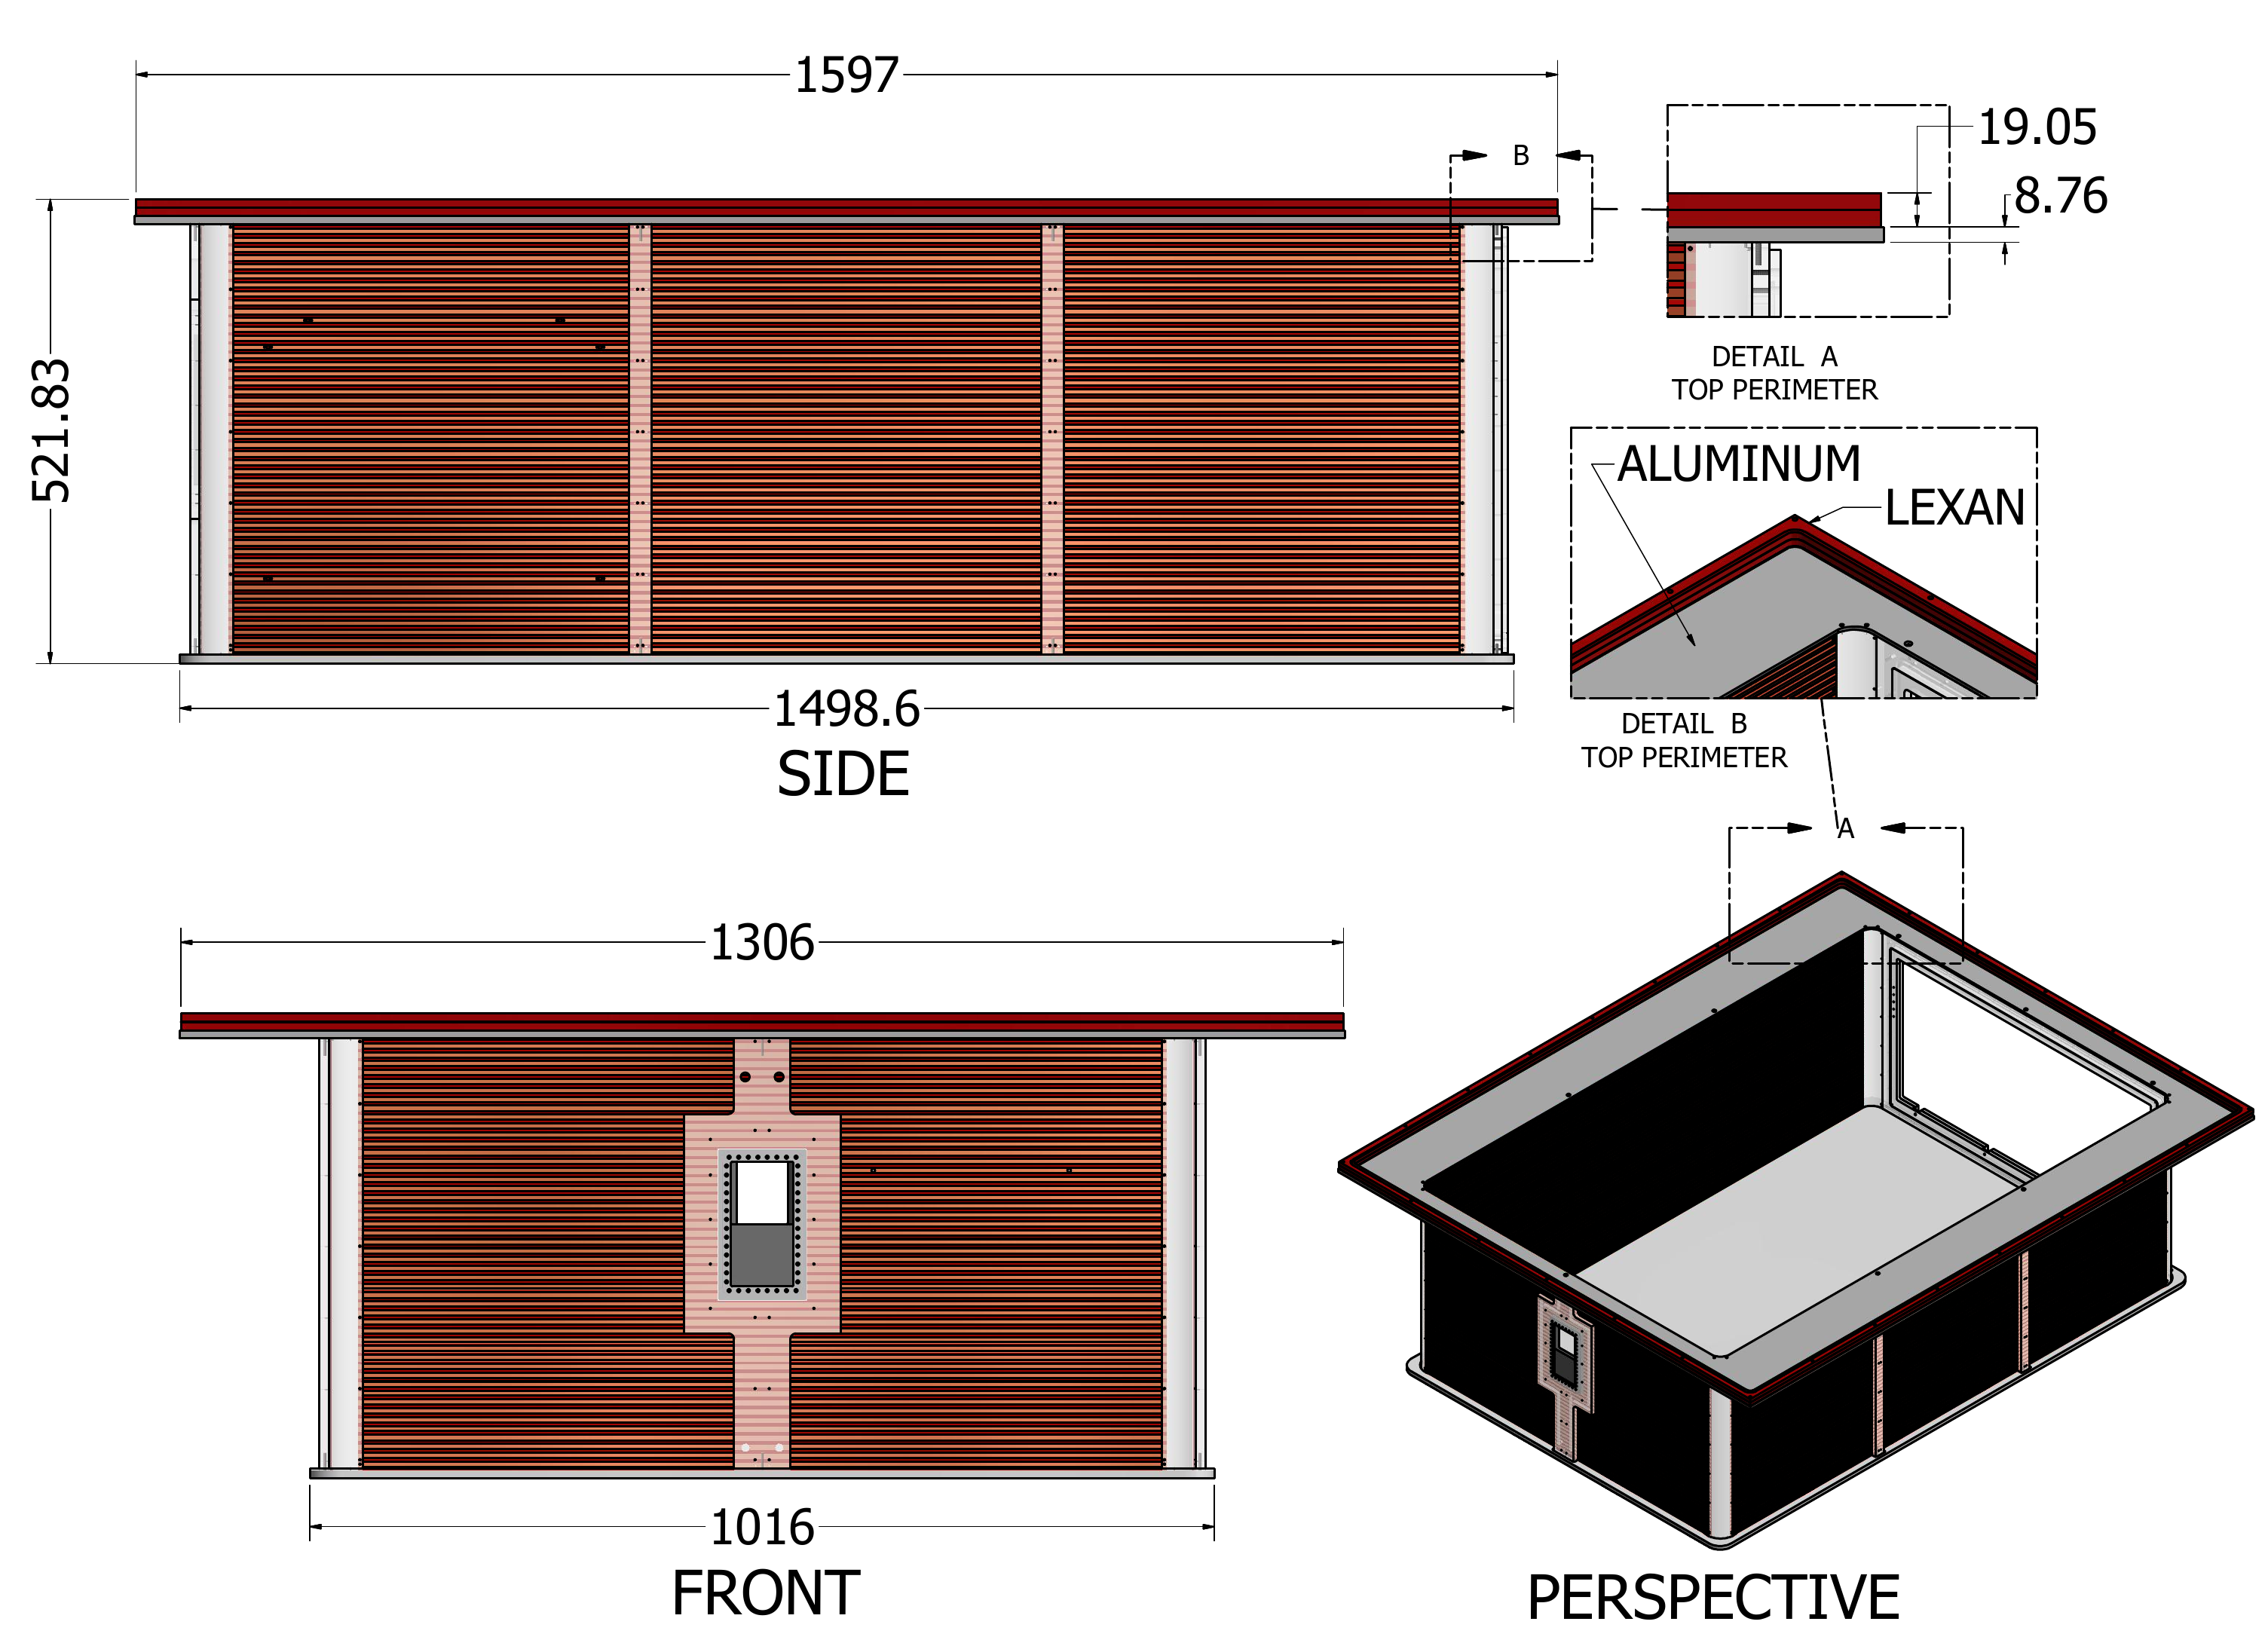
\includegraphics[width=\textwidth]{fc_overview2.png}
\label{fig:fc_overview2}
\caption{Schematic of the field cage.}
\end{figure}


The field cage was constructed from several panels of two-layer printed circuit board (PCBs). The front of the field cage was made of two PCBs and each side was constructed from three PCBs. These boards had copper strips etched onto the inside and outside of the board which when all the boards were assembed, formed copper rings which were used to set up the uniform electric field, as will be described later. The array of circuit boards were glued and supported by Lexan pieces. We did not use the common PCB substrate material FR4, which contains a Bromine impregnated epoxy which can outgas Bromine, which can absorb the secondary electrons from the track, thereby degrading the signal \cite{tpcAging}. Instead, a halogen free material, Cryogenic-G10, was used for the board material.  The downstream wall mainly consists of a large, thin exit window. The window  is constructed of   \SI{10}{\micro\metre} Kapton upon which are  evaporated aluminum strips that define the electric field. At the bottom of field cage is the cathode that is  constructed from an aluminum honeycomb laminate, composed of two aluminum sheets bonded to an aluminum honeycomb core, providing a lightweight yet rigid structure. On the other end the boards were epoxied into an aluminum top perimeter which also served as the last electrode ring in the TPC. Together with the cathode bottom, the field cage proved to be a rigid lightweight structure. A Lexan ring containing o-rings was placed in-between the top perimeter piece and the top plate of the TPC. Screws with nylon washers, and collars, were used to mount the top perimeter, and the field cage, to the top plate; it also provided electrical isolation from the top plate. In this way the top plate could be removed and rotated with the field cage attached, without damaging any internal components. 

\begin{figure}[!htb]
\centering
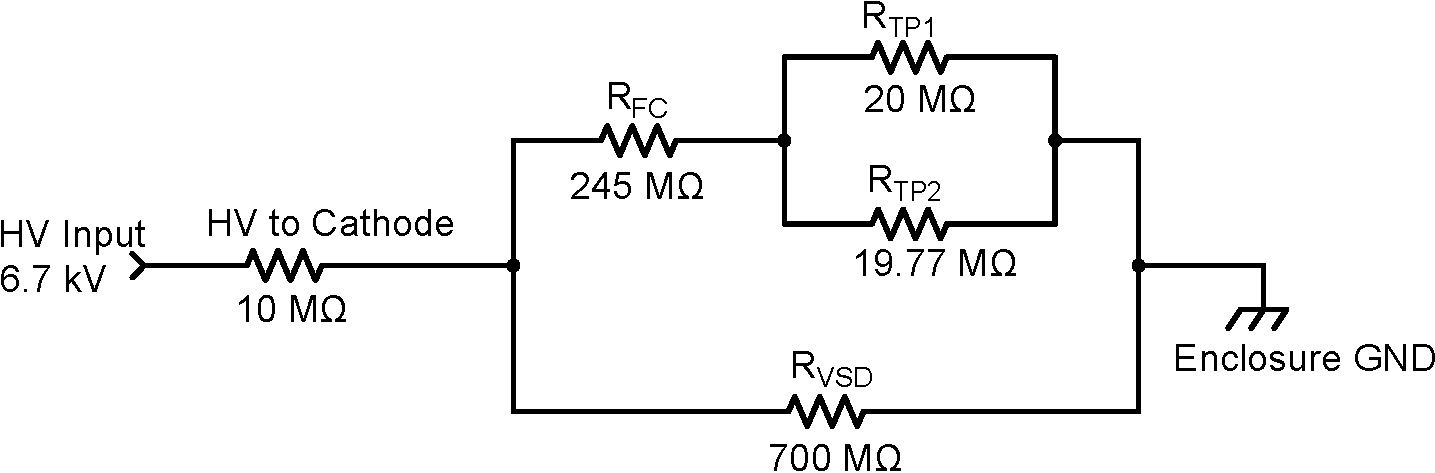
\includegraphics[width=\textwidth]{TPC_schematic.pdf}
\caption{Schematic of the resistive elements in the TPC system.}
\label{fig:TPC_schematic}
\end{figure}



Figure~\ref{fig:TPC_schematic} shows the schematic of the effective resistances and capacitance of the TPC subsystem. The cathode is connected to the high voltage (HV) supply through a \SI{10}{\mega\ohm} resistor and has an effective capacitance to ground of \SI{4}{\nano\farad}, $C_{VSD}$. The cathode voltage $V_{cath}$ can be calculated as,
\begin{equation}
V_{cath} = \frac{V_{HV}}{ 1 + \frac{10}{ \left( (245 + R_p)^{-1} + 700^{-1} \right)^{-1} } },
\end{equation}
where 
\begin{equation}
R_p = \left( R_{TP1}^{-1} + R_{TP2}^{-1} \right)^{-1},
 \label{eq:Reff}
\end{equation} 

is the effective resistance of the last resistor, and $V_{HV}$ is the high voltage supply; all resistor values are given in \si{\mega\ohm}.


\begin{figure}[!htb]
\centering
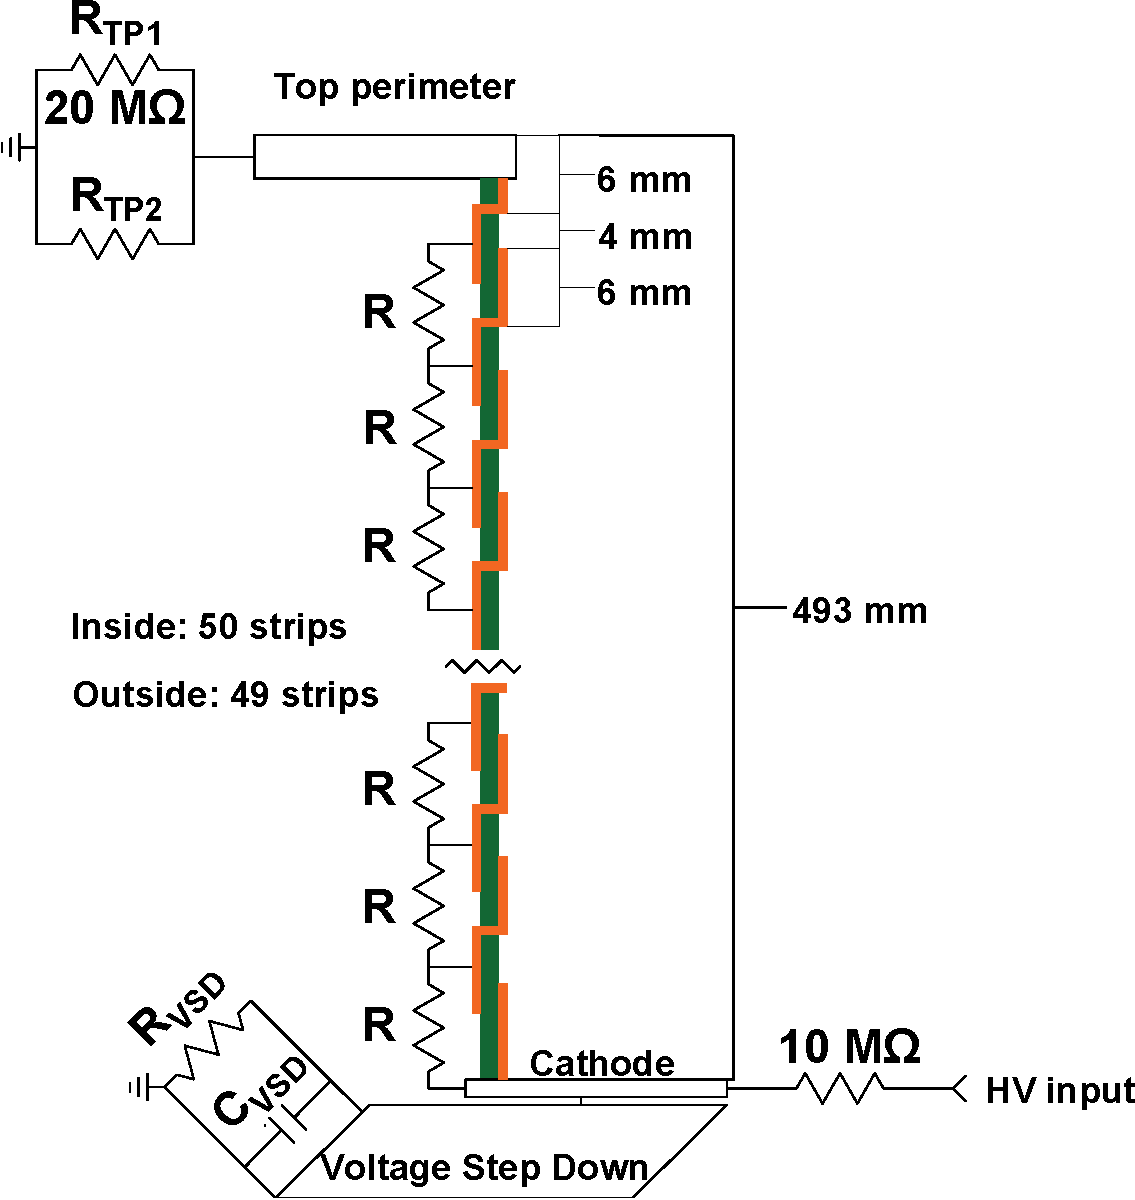
\includegraphics[scale=.6]{FC_schematic.pdf}
\caption{Schematic of the electric connections relevant to the field cage system. The strip thickness is exaggerated in the figure to show the detail.}
\label{fig:FC_schematic}
\end{figure}

Figure~\ref{fig:FC_schematic} shows a schematic detailing the connections involved in the field cage walls. The field cage contains 50 inside copper strips and 49 outside copper strips. The strips are \SI{6}{\milli\metre} in width and spaced \SI{10}{\milli\metre} apart. Since the field cage was build with an array of PCB boards, connections from adjacent strips were connected all the way around until all the strips formed a continuous ring. The interfaces were the side pieces met were connected by G-10 corner pieces where conductive paint strips were painted on. The first inside strip is connected to the cathode, which is itself connected by an effective \SI{5}{\mega\ohm} resistor ($R$) to the first outside strip. The first outside strip is connected through a via to the second inside strip. These outside strips formed a small electric field which repelled electrons away from the PCB substrate between inside strips, preventing build up on the insulating material. This pattern repeats until the very last strip. A resistor chain, connected to the outside strips, creates a voltage divider in which each strip is separated by a constant difference voltage and a fixed distance, setting up a constant electric field. The last strip of the field cage is composed of a small inner strip  (\SI{1.5}{\milli\metre}) on the PCB board and the top perimeter piece (\SI{4.5}{\milli\metre}) giving an  effective thickness of \SI{6}{\milli\metre}, which is the same as the other strip widths. The top perimeter is connected to electrical ground through a \SI{20}{\mega\ohm} resistor ($R_{TP1}$) with the option to place an additional resistor ($R_{TP2}$) in parallel to tune the voltage of the top perimeter, as seen in Figure~\ref{fig:FC_schematic}. Allowing for a tunable resistor allowed for fine tuning of the electric field in the region between the top perimeter and the wire planes as will be discussed in Section~\ref{sec:wireplanes}. 

The voltage on each strip, $V_n$, can be expressed as, 
\begin{equation}
V_n = V_{cath} \frac{R_p + (50 - n)R}{49\cdot R + R_p}
\label{eq:FCstrip}
\end{equation}

where $n = 1$ represents the index of the first inside strip, and $n= 50$ represents the index of the last inside strip, which is the same as the top perimeter voltage.



%Talk about the uniforminty of the field cage maybe
%how far the wall was from the pad plane on the sides talk about the front


\subsection{Voltage Step Down}
The gap between the cathode and the ground of the enclosure is quite small. To prevent electric breakdown in the gas between this gap, a series of concentric copper rings safely stepped down the voltage to ground in a controlled manner, reducing the chance of electric breakdown and sparking. There were 8 concentric rings with a \SI{10}{\mega\ohm} resistors in between, creating a resistor chain which steps down the voltage each ring by approximately \SI{1000}{\volt} each time. The first ring is the same voltage as the cathode and the last ring is connected to ground. All together the total resistance of the resistor chain is \SI{700}{\mega\ohm}.


\subsection{Wire Planes}
\label{sec:wireplanes}
%Add figure of gating grid transparency closed and open configuration 

There are three wire planes that are mounted underneath the pad-plane. The wire plane closest to the pad-plane (\SI{4}{\milli\metre}) are the anode wires. The next plane (\SI{8}{\milli\metre}) is the ground plane or Frisch grid. The last plane (\SI{14}{\milli\metre}) is the gating grid. The gating grid is the first plane that electrons meet as they drift upward from the field cage volume towards the anode plane. The gating grid functions as a gate, either allowing electrons and ions through, or blocking them entirely. The ground plane functions to shield the inside volume of the TPC from the high electric field surrounding the anode wires. The ground plane is the least interesting plane and is held to ground by shorting the plane to the enclosure ground through shorted BNC terminator on the outside of the TPC. We also use the ground plane to input a pulser, which is used to spread the pulsed signal to all the pads on the TPC in order to calibrate the electronics of the TPC. This is done by replacing the shorted BNC with a \SI{50}{\ohm} termination and injecting the pulser on the other end. 


 \begin{table*}[!htb]
 \centering
\ra{1.3}
\begin{tabular}{@{}rrrrrrr@{}}\toprule 
\multicolumn{2}{c}{GET electronics settings}\\
\midrule
 Plane & Material & Diameter \si{\micro\metre} & Pitch \si{\milli\metre} & Distance to pad-plane & Tension \si{\newton} & Voltage \si{\volt}\\ [0.5ex] 
 Anode  & Au-plated W   &  20  &  4  &  4   &  0.5  &  1460  \\
 Ground & BeCu          &  75  &  1  &  8   &  1.2  &  0     \\ 
 Gating & BeCu          &  75  &  1  &  14   &  1.2 &  -110$\pm$ 70\\ 
 \bottomrule
\end{tabular}
\caption{Wire plane properties.}
\label{tb:wireplane}
\end{table*}

In the open configuration, the gating grid is transparent to electrons coming from the field cage volume and also allows for ions to move from the avalanche region into the TPC volume. In the closed configuration it is opaque to electrons and ions, when set to the right voltages. Typically the gating grid is always in the closed configuration, only opening it momentarily when the data acquisition trigger criteria is met to take data. By keeping it always closed the electrons which come from the un-reacted beam are blocked,  which if allowed to go to the anode wires, would quickly build up enormous amounts of positive ions, which would flood the field cage with space charge, distorting the electrons represnting the track paths. We open the gating grid for about \SI{11}{\micro\second} which is more than the time it takes for the electrons to drift one TPC volume. After this, we close the gating grid to prevent the back-flow of ions from the avalanche region from that event. Since ions move with a velocity much slower than that of electrons \cite{blumrol}, the ions only move several \si{\micro\metre} in the time the gate is open. This allows for electrons to pass through while preventing the back-flow of ions into the FC volume, reducing or even eliminating the space charge resulting from the avalanche region.

Figure~\ref{fig:gg_onoff} shows a Garfield simulation of the drift lines of electrons in both the on and off configurations. In the on configuration, all the wires share the same average voltage, $V_{g.g.}$, which is set to the optimal voltage that represents of 100\% electron transparency. Figure~\ref{fig:wires_open} shows the electrons are allowed to drift completely through the gating grid all the way to terminate on the anode wires. In the off configuration, the reference voltage $V_{g.g.}$ remains the same, but alternating wires get an offset voltage of $\pm \Delta V$, so that the electric field produced by the voltage difference $2\Delta V$ between wires is great enough to block incoming electrons. Figure~\ref{fig:wires_closed} shows this case were the electron drift lines are fully blocked, as they terminate on the more positive wires. Opening the grid from this closed bi-polar mode is simply done by removing the offset voltage and allowing the two wires to short which equilibrates their charges, coming back to the average voltage setting in the on configuration.

\begin{figure}[!htb]%
    \centering
    \subfloat[Wires open]{{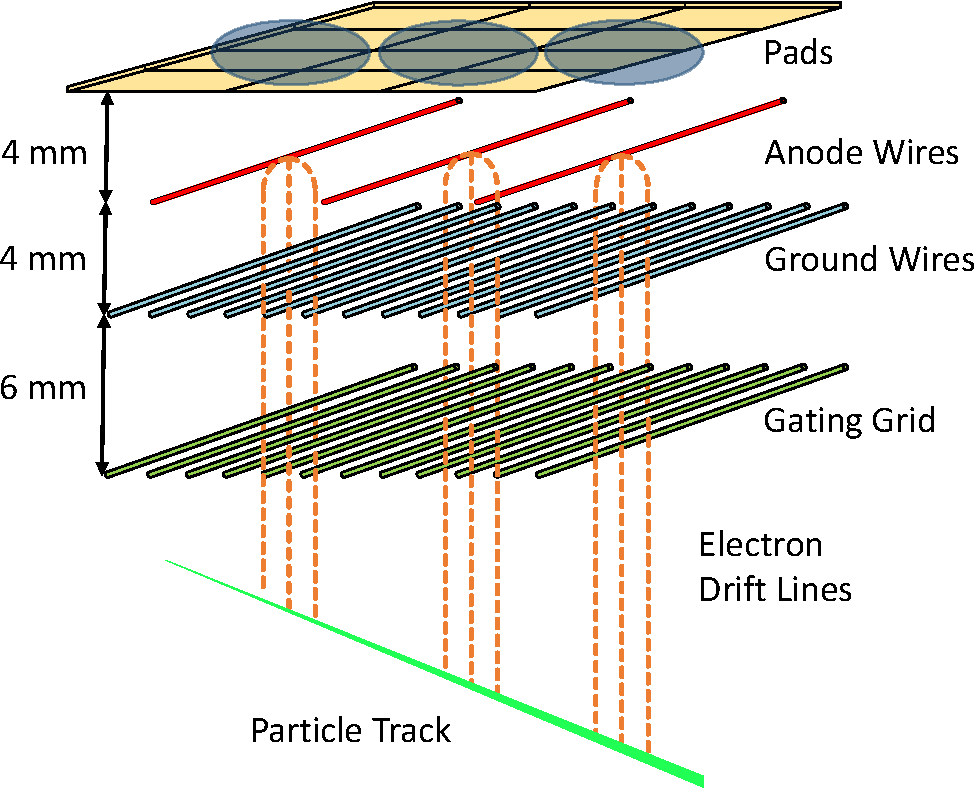
\includegraphics[width=.45\textwidth,valign=t]{wires_open.pdf} \label{fig:wires_open}}}%
    \qquad
    \subfloat[Wires closed]{{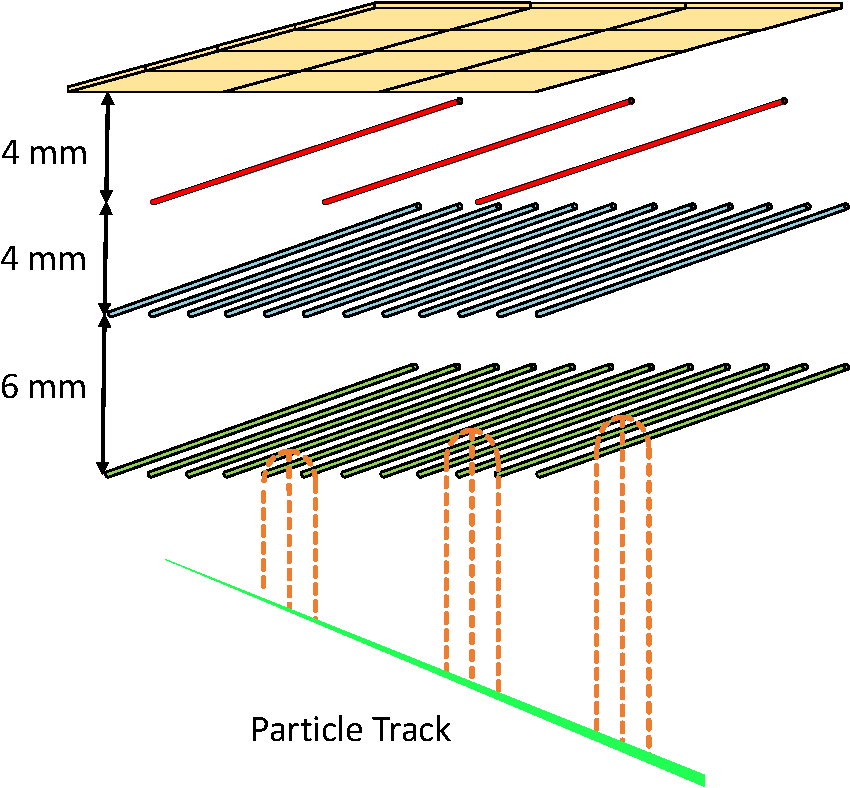
\includegraphics[width=.39\textwidth,valign=t]{wires_closed.pdf} \label{fig:wires_closed}}}%
    \caption{Cartoon depiction of electron drift lines going through the various wire planes.}%
    \label{fig:wires}%
\end{figure}

\begin{figure}[!htb]
\centering
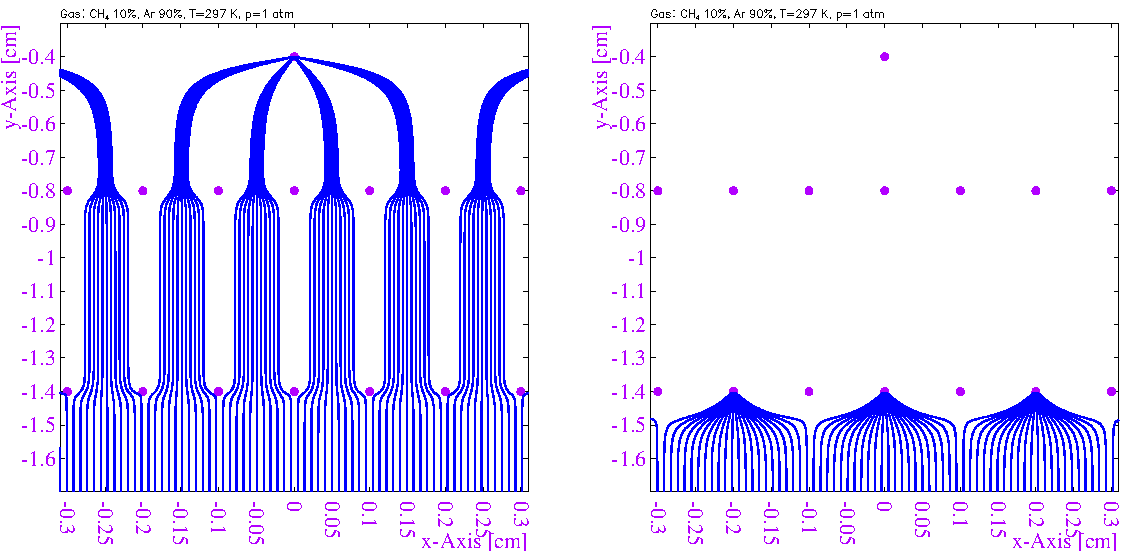
\includegraphics[width=\textwidth]{gg_onoff.pdf}
\caption{Garfield simulations of the on and off configuration of the gating grid.}
\label{fig:gg_onoff}
\end{figure}


Both configurations of the gating grid were measured and simulated. To measure the electron transparency in the on configuration all wires were set to the same voltage $V_{avg}$, and the anode wires were lowered to \SI{500}{\volt}. By lowering the voltage of the anode wires we could measure the large charge of the beam without saturating the electronics. The average charge deposited in the chamber was measured as a function of $V_{avg}$. Changing the average voltage required a different top perimeter resistor value according to Eq.~\ref{eq:TP_resistor}. Several runs were taken ranging from \SIrange{-198}{-40}{\volt}, with and without the magnetic field. Theoretically the most negative value represents 100\% electron transparency and was used as the reference run in which we scaled all measurements to. The measured electron transparency, $T$, was estimated as $T = \langle dE/dx\rangle/{\langle dE/dx\rangle}_{ref}$, where $\langle dE/dx\rangle_{ref}$ represents the average energy loss of the reference run. Figure~\ref{fig:ggAvgTrans} shows the measured transparency as a function of $V_{avg}$, as compared with the corresponding Garfield simulation \cite{garfield++}. The average gating grid voltage used in the experiment was \SI{-171}{\volt} to ensure we were well within the 100\% transparency region. 

To measure the electron transparency as a function of the difference voltage $\Delta V$, the average voltage was first set to 100\% transparency, $V_{avg}=\SI{-171}{\volt}$, and the difference voltage was added and subtracted from alternating wires. Figure~\ref{fig:ggDeltaVTrans} shows the result of the simulation and experiment with and without the magnetic field. By introducing the magnetic field the required voltage to close the grid increased as expected. In the experiment we selected the value of $\Delta V = \SI{65}{\volt}$ to ensure we were well within the region of 0\% transparency. In both the on and off configurations good agreement was seen with the corresponding Garfield++ simulations when accounting for statistical error in the MC simulations and in the data.   



\begin{figure}[!htb]%
    \centering
    \subfloat[On configurations where all wires are the same voltage.]{{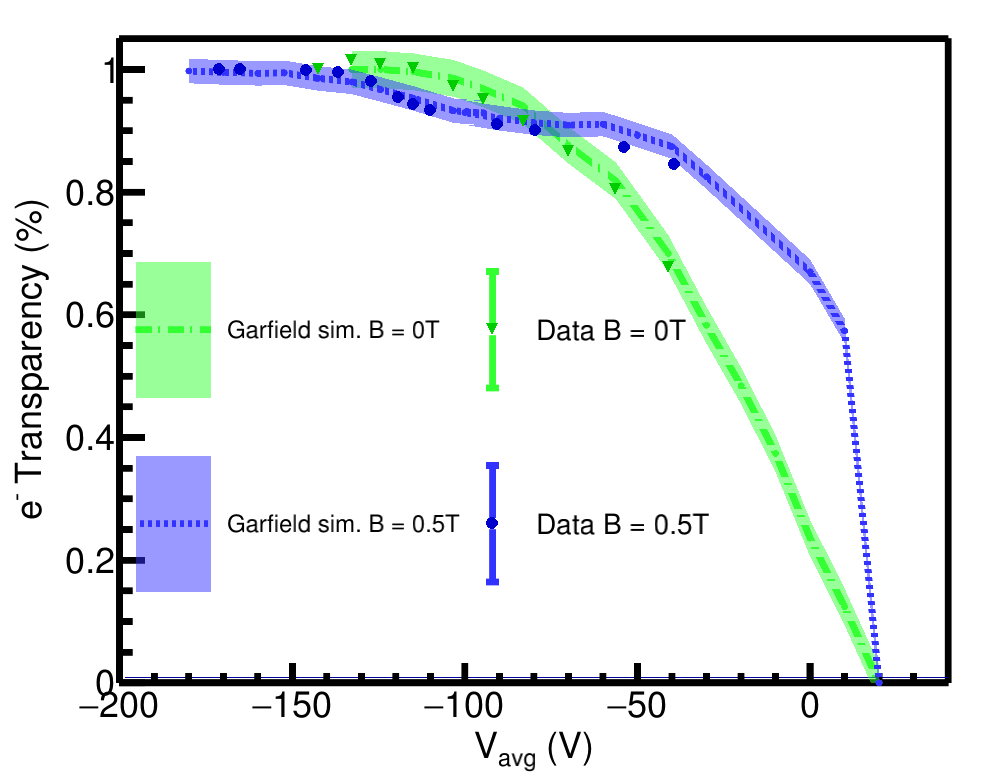
\includegraphics[width=.45\textwidth,valign=t]{averageTransparency.png} \label{fig:ggAvgTrans}}}%
    \qquad
    \subfloat[Off configuration where adjacent wires have a voltage difference of $2 \Delta V$.]{{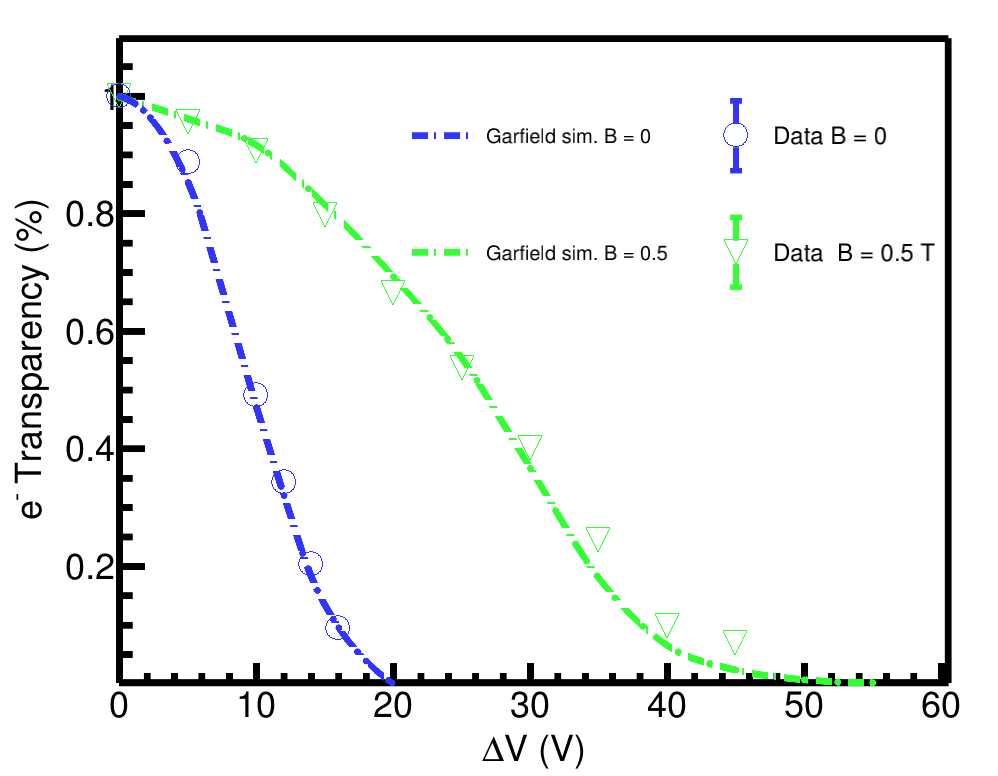
\includegraphics[width=.45\textwidth,valign=t]{transparencyDeltaV.png} \label{fig:ggDeltaVTrans}}}%
\caption{Electron transparency as measured and simulated in the on and off configurations of the gating grid.}    
\label{fig:ggTrans}
\end{figure}


The anode wires are made of very thin Gold plated Tungsten wires, about \SI{20}{\micro\metre} in diameter. They are biased to high voltages of about  \SI{e3}{\volt} which creates a very high electric field very close to the anode wire. As the electron approaches the anode wire, the field gets strong enough that the kinetic energy gained between collisions exceeds the ionization potential of the gas nocking out more electron-ion pairs in the gas. This happens over several collisions creating an avalanche effect amplifying the electron current.  The final number of electrons produced depends on the anode wire voltage and the gas properties. The absolute gas gain was not experimentally determined but it was calculated in a Garfield simulation. For the experimental data pertaining to this disertation, the anode wires were biased to two different voltages. We will refer to the voltage \SI{1460}{\volt} as the \emph{high voltage} and \SI{1214}{\volt} as the \emph{low voltage}. Two sections were biased with the lower voltage setting to minimize the effects of a leakage of secondary electrons around the end of the gating grid \cite{jon}.


 Figure~\ref{fig:anodegain} shows the electron distribution for the total number of electrons produced in a avalanche process created by a single electron. The distribution follows the expected Polya distribution, and the MC data in the simulation was fitted with a Polya function \cite{blumrol}, which can be expressed as,

\begin{equation}
P(x) = A_0^{-1}\cdot \frac{A_1^{A_1}}{\Gamma(A_1)} \left(\frac{x}{A_0}\right)^{A_1-1}e^{\frac{-A_1x}{A_0}}.
\end{equation}

For the voltage of \SI{1460}{\volt} the parameters of the fit are $A_0=903.9$ and $A_1=1.50$ and for the voltage of \SI{1214}{\volt} the parameters are $A_0=150.0$ and $A_1=1.47$. These Polya distribution fits will be important later as the input to the Monte Carlo simulations of the detector response in Section~\ref{sec:monteCarlo}.



\begin{figure}[!htb]
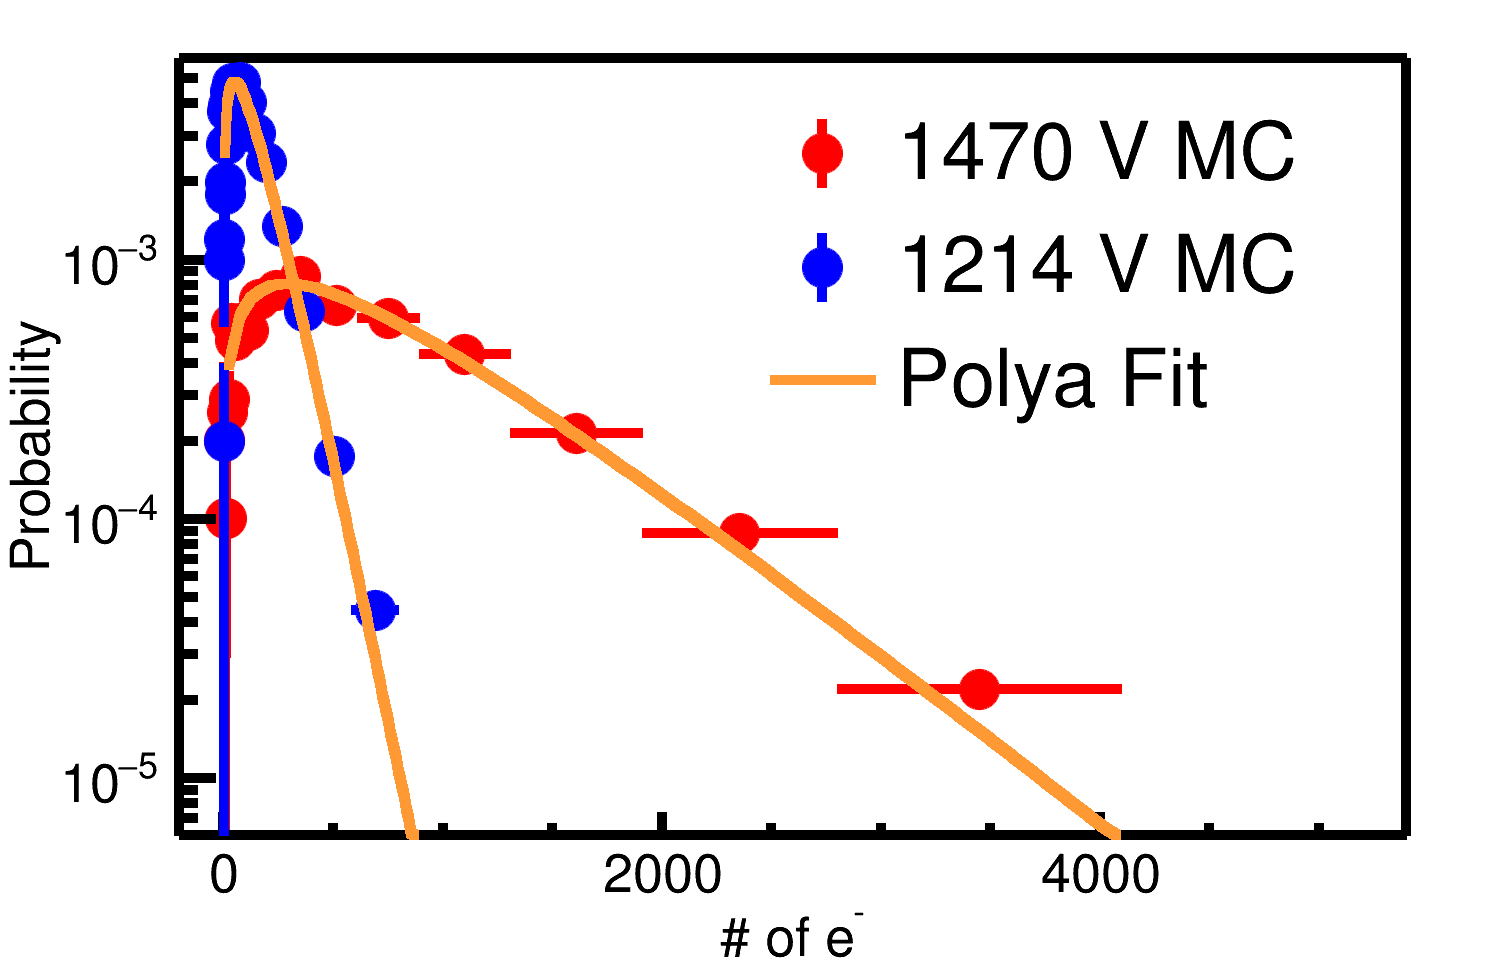
\includegraphics[width=\textwidth]{gain.png}
\caption{Number of electrons produced in a single avalanche on an anode wire. Two different voltages were simulated using Garfield++ at 1470 $V$ and 1214 $V$. The expected Polya distribution fit is also given in yellow.}
\label{fig:anodegain}
\end{figure}



Care must be taken to choose the resister ($R_{TP2}$) that connects the field cage divider chain to the top plate. The end of the field cage nearest to the top plate is at the same potential as the aluminum top perimeter piece to which the field cage is glued. This top perimeter piece forms a horizontal surface that is an equipotential representing the last ring. The voltage difference between the average voltage on  the gating grid and the voltage of the top perimeter influences the electric field just below the gating grid. If $R_{TP2}$ is incorrectly chosen, the electric field near the gating grid will be different for electrons that pass near the field cage walls than it is for electrons in the center of the TPC,  causing distortions of the tracks in the TPC. This requires the value for $R_{TP2}$ to be chosen correctly. Since this simple point can be easily forgotten, we now discuss this choice in greater detail.

To understand how to calculate $R_{TP2}$ we imagine the space between the cathode and the gating grid can be split into two virtual volumes, Region 1 defined as the space between the cathode and the top-perimeter, and Region 2 defined between the top-perimeter and the gating-grid. The magnitude of the electric field in the region between the top-perimeter and the cathode, $E_1$, is defined as,

\begin{equation}
E_1 = \frac{V_{g.g.} - V_{tp}}{ y_{g.g.} - y_{tp} },
\end{equation}
where  $V_{g.g.}$, $V_{tp}$ , $y_{g.g.}$, and $y_{tp}$ are the voltages and vertical y-positions of the gating-grid and top-perimeter respectively. The y-position here refers to the center of the electrodes. The magnitude of the electric field in the region between the top-perimeter and the cathode, $E_2$, is defined as,

\begin{equation}
E_2 = \frac{V_{tp} - V_{cath}}{ y_{tp} - y_{cath} },
\end{equation}
where  $V_{tp}$, $V_{cath}$ , $y_{tp}$, and $y_{cath}$ are the voltage and vertical y-position of the top-perimeter and cathode respectively. The y-position of the cathode is defined as the face of the cathode. The condition for a smooth electric field across these two virtual volumes is defined as the solution to the equation $E_1 = E_2$. Substituting Eq.~\ref{eq:FCstrip} for $V_{tp}$ -- $n=50$ -- we can solve for the effective resistance of the top perimeter $R_p$ as, 

\begin{equation}
R_p = 49 \cdot R  \left(\frac{ y_{g.g.} - y_{cath} }{ y_{TP} - y_{cath} \frac{V_{cath} - V_{gg}}{V_{cath}} }- 1 \right),
\label{eq:TP_resistor}
\end{equation}

where the relevant vertical dimensions are $y_{g.g.} - y_{cath} = \SI{497.3}{\milli\metre}$ and $y_{tp} - y_{cath} = \SI{490}{\milli\metre}$. The value of $R_{TP2}$ can then be calculated from Eq.~\ref{eq:Reff}.


\subsection{Pad Plane}
The pad-plane is a multi-layer circuit board which is segmented into \SI{11.5}{\milli\metre} x \SI{7.5}{\milli\metre} charge sensitive pads, arranged in an array of 108 x 112 pads in the x and z-directions respectively; making 12096 pads in total. There is an insulating gap of \SI{0.5}{\milli\metre} on each side separating the pads so that the effective area covered by the pads is \SI{1344}{\milli\metre} x \SI{864}{\milli\metre}. There is a via and trace coming from each pad, through the board, to the opposite side of the pad plane, and is arranged in a surface pads which is readout by a surface mount SAMTEC connector. Figure~\ref{fig:padplane} shows the pad plane boards being glued to the top plate and the holes which allow for the readout of pads. The pads were gold plated for excellent electric conduction properties. 

\begin{figure}[!htb]
\centering
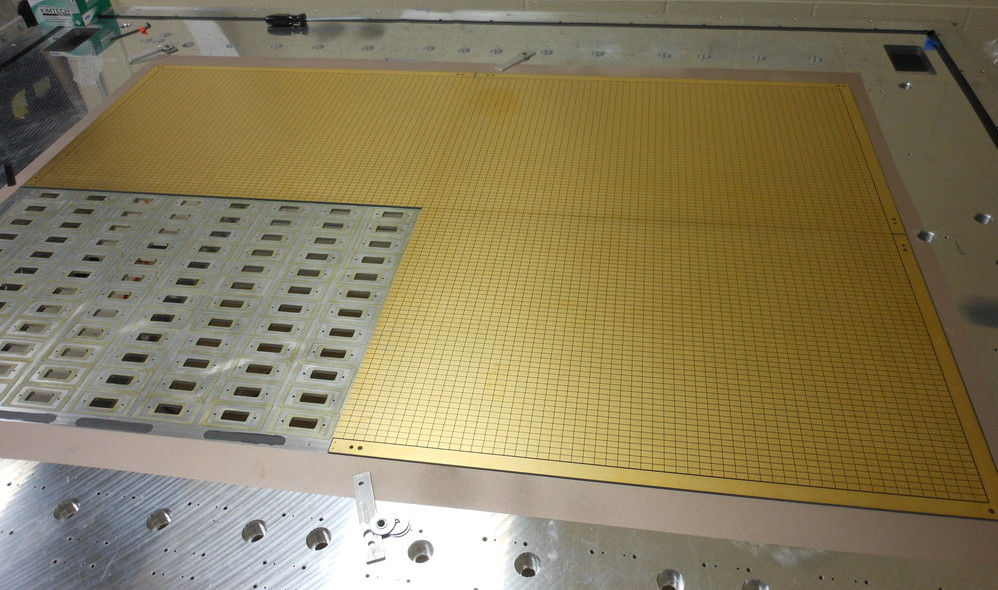
\includegraphics[width=\textwidth]{3boards_ps.jpg}
\caption{Figure of the pad plane boards being glued to the top plate. }
\label{fig:padplane}
\end{figure}


\subsection{Electronics}

Signals in the S$\pi$RIT TPC are amplified and digitized by the recently developed Generic Electronics for TPCs (GET) \cite{get}.  Short cables transmit the signals from the surface mount connectors, through a circuit protection board called ZAP, to the inputs of the AGET chips which are mounted to the AsAd board as seen in Figure~\ref{fig:getzap}. Each AGET chip services 64 pads (63 pads are connected in our case). Four AGET chips are mounted on one AsAd  motherboard. Figure~\ref{fig:aget} is the schematic of each  AGET chip which contains a charge sensitive pre-amplifier, several other stages of amplifiers, and a Switched Capacitor Array (SCA) with a maximum of 512 time buckets which operates in a circular readout buffer. The sampling frequency can be adjusted from 1 to \SI{100}{\mega\hertz}. The gain of each AGET can be configured as 0.12, 0.24, 1.0, or \SI{10}{\pico\coulomb} over the whole dynamic range, and the analog-to-digital converters (ADCs) on each AsAd board provides 12 bit resolution. The peaking times of the shaping amplifiers can be set to 69, 117, 232, 501, 720, or \SI{1014}{\nano\second}. In this experiment, the gain was set to the highest setting, 0.12 \si{\pico\coulomb}, the peaking time \SI{117}{\nano\second}, and the sampling frequency \SI{25}{\mega\hertz} (resulting in \SI{40}{\nano\second} time buckets). 

\begin{table*}[!htb]
\centering
\ra{1.3}
\begin{tabular}{@{}rr@{}}\toprule 
\multicolumn{2}{c}{GET electronics settings}\\
\midrule
ADC bit range       & 14 bits \\
Sampling frequency  & 1-100 MHz \\
Dynamic range       & .12, .24, 1.0, 10pC \\
Peaking time        & 69,117,232,501,720,1014 ns \\
Time bucket range   & 512\\
\bottomrule
\end{tabular}
\caption{Summary of range of GET electronics settings. }
\label{tb:getoverview}
\end{table*}

\begin{figure}[!htb]
\centering
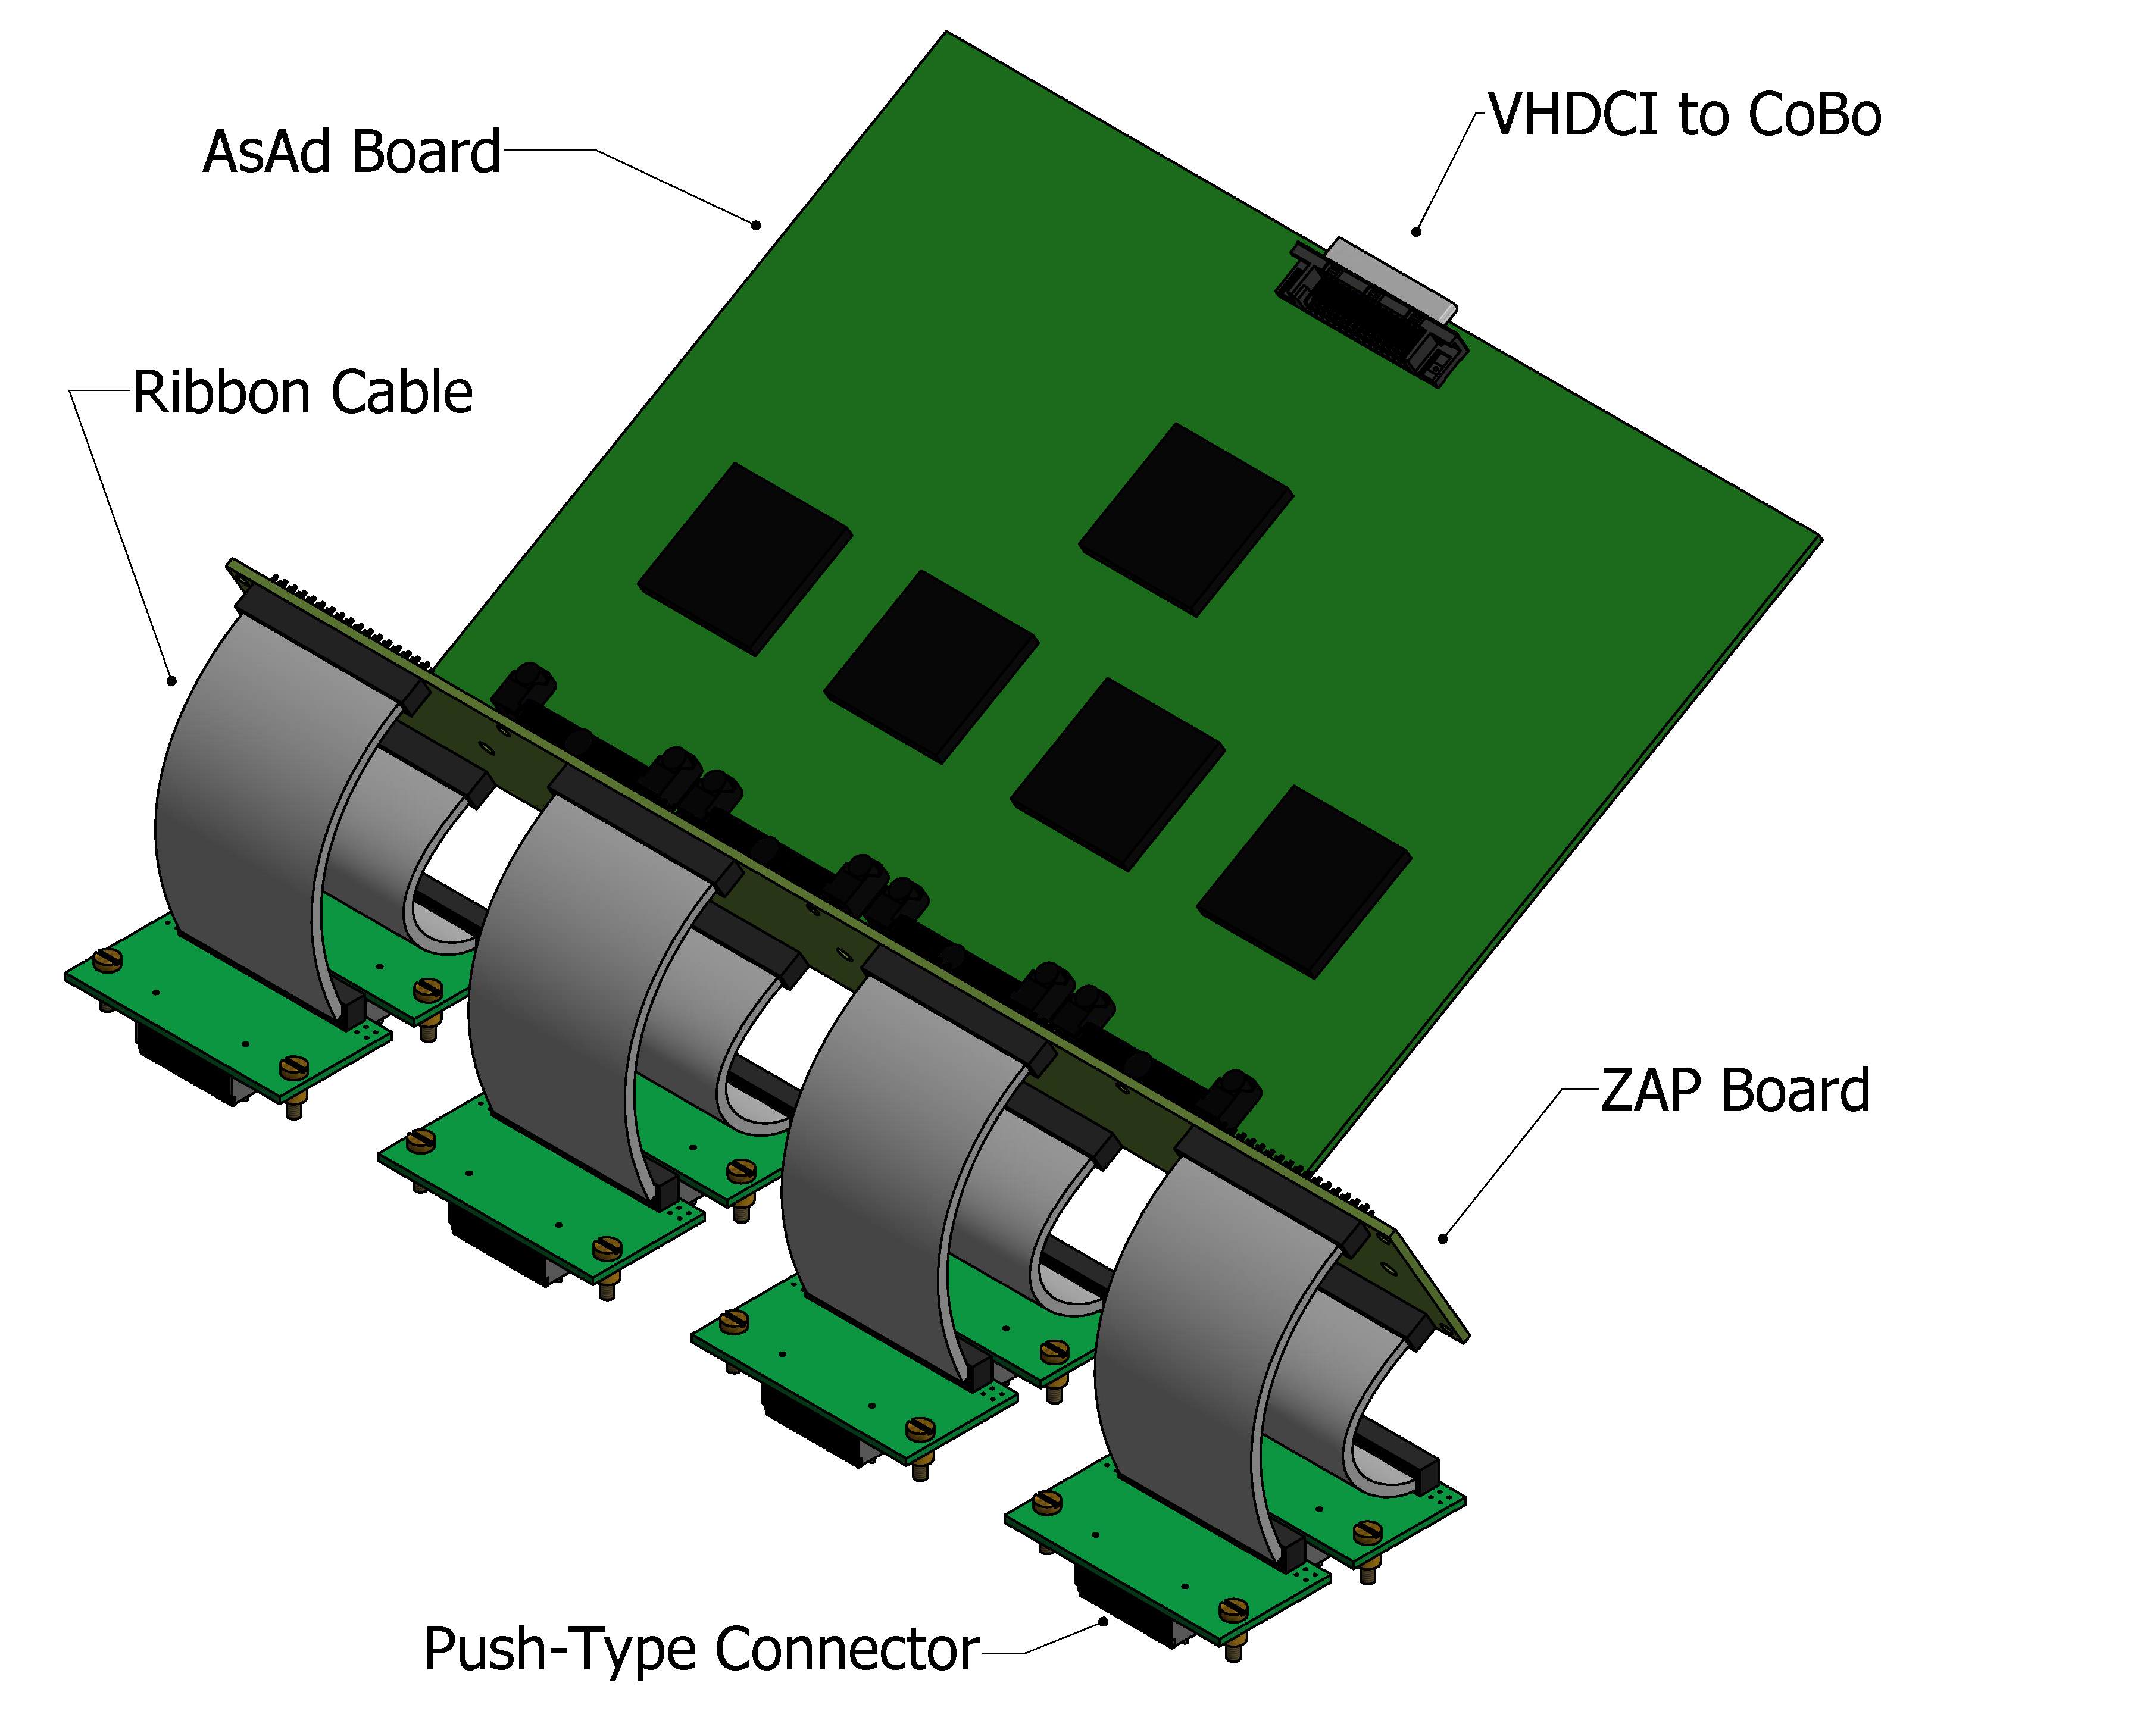
\includegraphics[width=.5\textwidth]{GET_and_ZAP.pdf}
\caption{Drawing of the ZAP and AsAd board which is connected to the surface pads on the backside of the pad-plane.}
\label{fig:getzap}
\end{figure}



\begin{figure}[!htb]
\centering
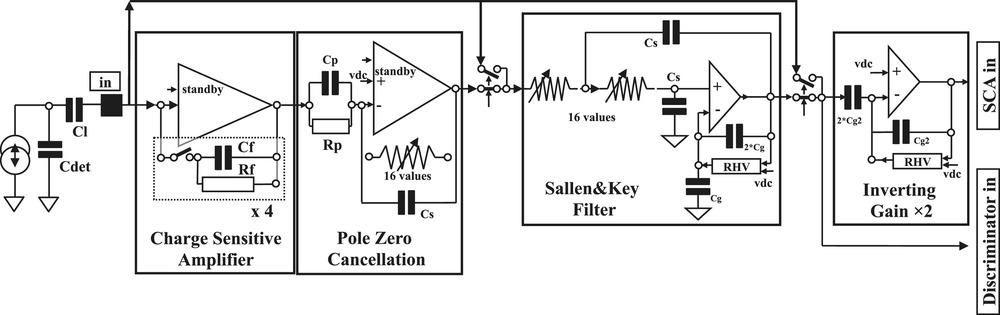
\includegraphics[width=\textwidth]{AGETfncn.jpg}
\caption{Schematic of the internals of the AGET chip from \cite{get2}}
\label{fig:aget}
\end{figure}


\begin{figure}[!htb]
\centering
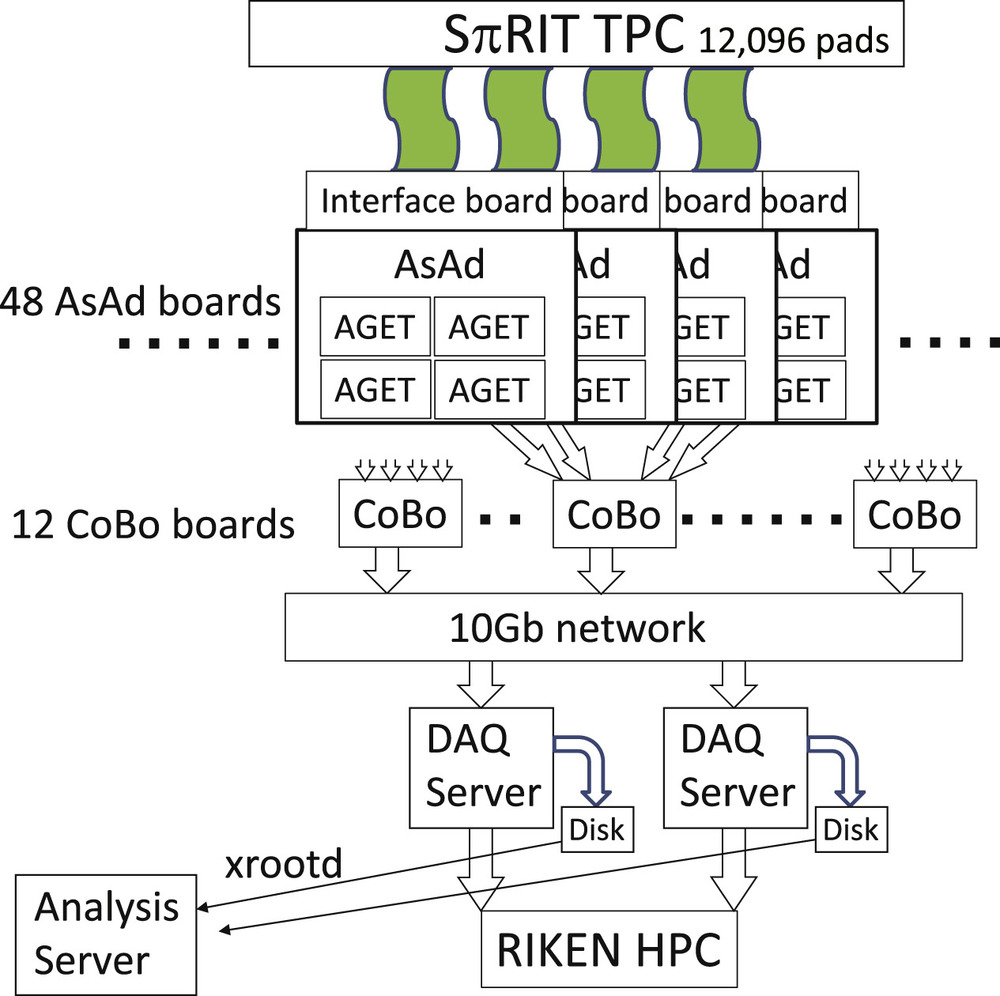
\includegraphics[width=.5\textwidth]{GETlayout.jpg}
\caption{Readout structure of the AsAd boards and CoBo board structures. Also the relevant components of the DAQ system.}
\label{fig:coboDAQ}
\end{figure}

After each AsAd board has digitized the data it is sent to the Concentration Boards (CoBo). Each CoBo board can concentrate the data from 4 AsAd boards. The Multiplicity, Trigger, and Time module (MuTanT) \cite{get} provides the common trigger signal for all CoBo boards.  Each board sends the data to the DAQ server which writes to disk the data from each board, which was handled by two separete DAQ servers; saving to one common analysis server. The data could then be analyzed using the RIKEN High Performance Computing (HPC) cluster or moved to the NSCL or MSU cluster for analysis. The Aget 2.0, asad 2.1, and cobo 1.0 firmware versions were used in this analysis. 

\section{Energy loss in material}
\label{sec:energyloss}

The average energy loss in a material can be described by the Bethe-Bloch equation,
\begin{equation}\label{eq:bb}
\frac{dE}{dx} = \frac{4\pi NZ^2e^4}{mc^2\beta^2} (\ln \frac{2mc^2\beta^2\gamma^2}{I} - \beta^2),
\end{equation}
where $N$ is the number density of electrons in the medium, $e$ the elementary charge, $mc^2$ is the rest mass of the electron, $Z$ is the charge of the traversing particle, $I$ is the mean excitation energy of the medium, and $\beta$ is the velocity of the particle \cite{blumrol}. Yet there is a large variation in energy loss around this mean value. The statistical variation of energy loss in a material was described by Landau \cite{landau} and later better described by Shulek \cite{shulek} and Bichsel \cite{bichsel1}. In both approximations it is described by a most probable energy loss value, with a long, high-energy loss tail. The solid curve in Figure~\ref{fig:straggling} shows the energy loss distribution in Ar gas for a proton with momentum \SI{3.4}{\giga\eVperc} \cite{bichsel}. The dashed line is the distribution under the Landau assumptions. The mean energy loss $\langle\Delta\rangle$ is significantly shifted from the most probable value $\Delta_p$, due to the long high energy tail.  Because of this long tail, for a finite set of energy loss measurements along a given track, the mean value is a very unreliable. The most probable energy loss is the better observable which can be obtained either through fitting of the observed distribution or through the truncated mean method. 

\begin{figure}
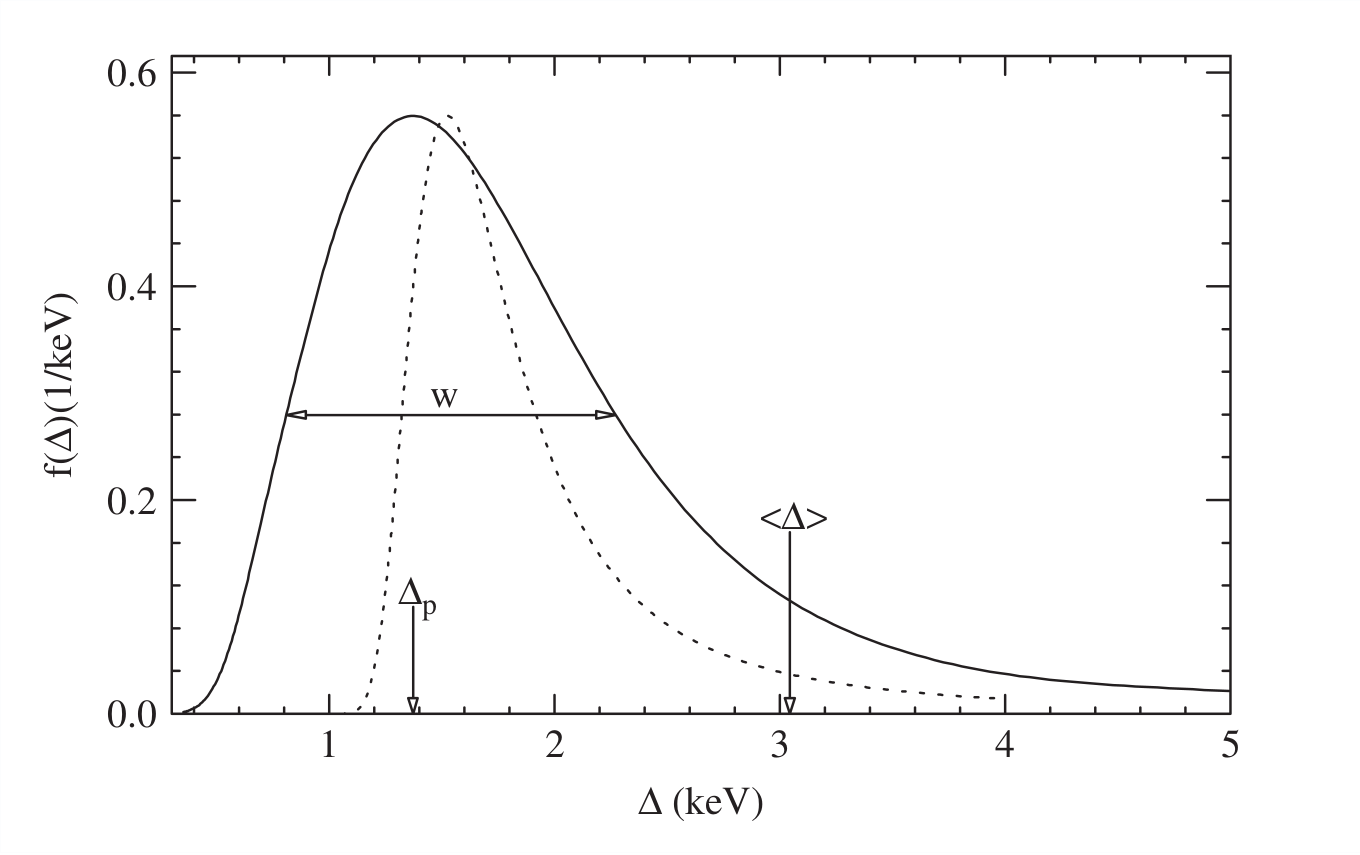
\includegraphics[width=\textwidth]{bichsel.png}
\caption{Energy loss distribution of a $\beta\gamma$ = 3.6 particle in Ar gas taken from \cite{bichsel}}
\label{fig:straggling}
\end{figure}

The truncated mean is the average mean value calculated after throwing away the top fraction of the highest energy loss entries. This approximates the most probable value without performing a fit to a known distribution. If a set of $n$ observed energy loss values, $\Delta_i/x$, in a given track are sorted from smallest to largest value. The truncated mean $C$, is calculated from the reduced set of points $n_t = f_r n$ as,

\begin{equation}
C = \frac{1}{n} \sum\limits_{i}^{n_t} \Delta_i/x,
\label{eq:truncmean}
\end{equation}

where $f_r$ is the cut off fraction. In this thesis, a value of 0.7 was used and it was also used in the STAR TPC collaboration \cite{starsyst}. 




%Suppose $E$ represents the set of $N$ energy loss points measured, sorted from lowest to highest energy loss. The $j^{th}$ index marks the position where  $i > j$ entries represent the highest value of energy loss measurements, where their fraction of the total set is expressed as, $f_c = \sum_{i>j} E_i/ \sum_i E_i$. The truncated mean is expressed as the mean value of the remaining energy loss measurements, throwing away the top $f_c$ fraction, expressed as,

%\begin{equation}
%\langledE/dx\rangle_t = \frac{\sum_{i < j} E_i}{N}
%\label{eq:truncatedM}
%\end{equation}

 %A full description of the energy loss distribution can be described in CITE HERE.


\subsection{Gas Properties}
The gas used was a mixture of 90\% Ar and 10\% Methane ($\mathrm{CH_4}$) by volume (P10 gas), and operated just under atmospheric pressure 1 atm. The gas was continually flowed through the field cage and exited into the enclosure volume, finally passing through a bubbler to atmosphere. The gas purity was monitored with an oxygen and water monitor which are the two most concerning contaminants. The water never exceed  100 ppm  and the oxygen level never exceeded 10 ppm, which are the two main contaminants in the gas which can absorb primary electrons \cite{tpcAging}. Figure~\ref{fig:driftvel} shows the drift velocity of P10 gas at 1 atm (\SI{760}{\torr}) as a function of the reduced electric field value given in units of \si{\volt\per\centi\metre\per\torr}. Operating near the peak value of the drift velocity curve minimized the change in the drift velocity as the effective field slightly changes due to slight variations in the pressure. The electric field in the experiment was \SI{125}{\volt\per\centi\per\metre} at \SI{760}{\torr}, giving a reduced electric field \SI{0.17}{\volt\per\centi\metre\per\torr}.

\begin{figure}[H]
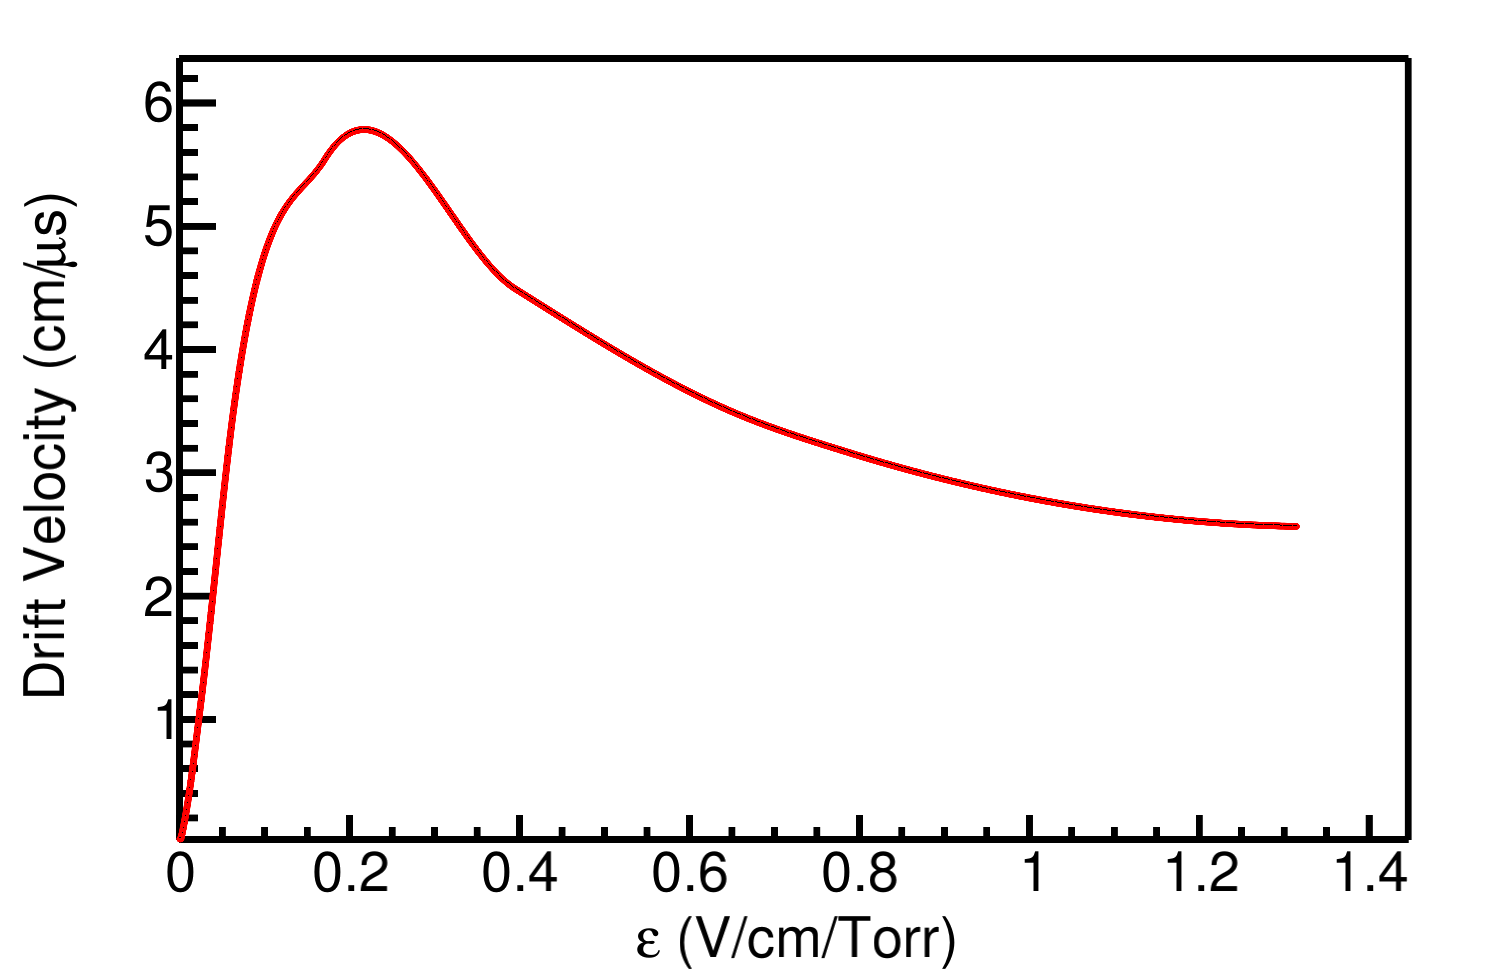
\includegraphics[width=\linewidth]{driftvel.png}
\caption{Drift velocity of electrons in P10 gas as a function of the reduced electric field.}
\label{fig:driftvel}
\end{figure}

The general formula for the drift velocity, $d\vec{x}/dt$, of an electron in the presence of electric and magnetic fields, $\vec{E}$ and $\vec{B}$, can be expressed in the Langevin equation as,  

\begin{equation}
\frac{d\vec{x}}{dt} = \frac{\mu}{1+(\omega\tau)^2}\Big(\vec{E} + \omega\tau\frac{\vec{E}\times\vec{B}}{|\vec{B}|}+\omega^2\tau^2\frac{\vec{E}\cdot\vec{B}}{|\vec{B}|^2}\vec{B}\Big),
\label{eq:elecdrift}
\end{equation}

where $\mu=\SI{5.43}{\centi\metre\per\second}$ is the signed drift velocity, $\omega=\SI{8.79e10}{\radian\per\sec}$ is the cyclotron frequency, and $\tau=\SI{2.48e-11}{\second}$ is the collision parameter for a particular gas \cite{blumrol}.

Several properties of the gas were simulated in Garfield including the longitudinal and transverse diffusion, $\sigma_l$ and $\sigma_t$ respectively, and the electron and ion drift velocities, $v_d$ and $v_i$ respectively for the experimental electric field of \SI{125}{\volt\per\centi\metre}. The results are summarized in Table~\ref{tb:gasprop}.


\begin{table}[!htp] % not just 'h!'
\centering % not a center environment
\begin{tabular}{
  @{}
  l
  S[table-format=1.2]
  S[table-format=1.2]
  S[table-format=1.2]
  S[table-format=1.2]
  S[table-format=5.2]
  S[table-format=5.2]
  @{}
}
\toprule
Gas properties &
 {$\sigma_{t}$} &
 {$\sigma_{l}$} &
 {$v_{d}$} &
 {$v_{i}$}  &
 {$G_{h}$} &
 {$G_{l}$} \\
&
  {($\si{\centi\meter}^{-1/2}$)} &
  {($\si{\centi\meter}^{-1/2}$)} &
  {(\si{\centi\meter\per\micro\second})} &
 {(\si{\centi\meter\per\micro\second})} \\

\midrule
\phantom{abc}   &.024   &.034  &5.43  &  \num{2.05e-4} &  903   &150     \\
\bottomrule
\end{tabular}

\caption{Gas properties of P-10 gas at 1 atm pressure.}
\label{tb:gasprop}
\end{table}

%Add table for gas diffusion 

\section{Pad Response Function}
\label{sec:prf}
Each electron avalanche produces an two-dimensional image charge on the pad plane, as shown in the cartoon in Figure~\ref{fig:2DPRF}, where the projection of the charge distribution onto the $x$ and $z$ axis of this distribution are labeled as $\rho(x)$ and $\rho(z)$ respectively. If $\rho(x,z)$ represents the charge distribution on the pad-plane, the total charge observed a particular pad, $Q$, is expressed as,

\begin{equation}
Q(x_o,z_o) = \int_{z_o - \frac{l}{2}}^{z_o + \frac{l}{2}} \int_{x_o - \frac{w}{2}}^{x_o + \frac{w}{2}} \rho(x-x_o\textprime,z - z_o\textprime) dxdz,
\label{eq:prfpadCharge}
\end{equation}

where $x_o$ and $z_o$ represent coordinates of the center of that pad, $x_0\textprime$ and $z_o\textprime$ are the coordinates of the avalanche, $w$ is the width, and $l$ is the length of the pad. The total charge observed for a given track is a superposition of all avalanches on all the anode wires. Typically in a TPC, the charges on each pad are grouped into clusters, and it is practical to cluster in only one direction. Therefore we will speak about the marginal probability distribution over a given layer of pads (x-distribution), or row of pads (z-distribution). The marginal distribution for a given layer can be written as,
\begin{equation}
\rho_x(x) = \int_{z_o - \frac{l}{2}}^{z_o + \frac{l}{2}} \rho(x,z)dz,
\end{equation}

and over a given row can be written as,

\begin{equation}
\rho_z(z) = \int_{x_o - \frac{w}{2}}^{x_o + \frac{w}{2}} \rho(x,z)dx.
\end{equation}

By substituting the variables  $\lambda_x = x - x_o\textprime$, and $\lambda_z = z - z_o\textprime$, we can express the charge distribution independent of the avalanche location. The Pad Response Function (PRF) along the x-direction of a given layer can be written as,

\begin{equation}
P_X(\lambda_{x_o}) = \frac{ \int_{\lambda_{x_o}-\frac{w}{2}}^{\lambda_{x_o} + \frac{w}{2}} \rho_x(\lambda_x)d\lambda_x } {\int_{-\infty}^\infty \rho_x(\lambda_x)d\lambda_x     },
\label{eq:prflayer}
\end{equation}

where $\lambda_{x_o} = x_o - x_o\textprime$; in a similar manner for the situation we cluster along the z-direction  of a given row the PRF can be written as,

\begin{equation}
P_Z(\lambda_{z_o}) = \frac{ \int_{\lambda_{z_o}-\frac{l}{2}}^{\lambda_{z_o} + \frac{l}{2}} \rho_z(\lambda_z)d\lambda_z }{\int_{-\infty}^\infty \rho_z(\lambda_z)d\lambda_z  },
\label{eq:prfrow}
\end{equation}

where $\lambda_{z_o} = z_o - z_o\textprime$.


\begin{figure}[!htb]
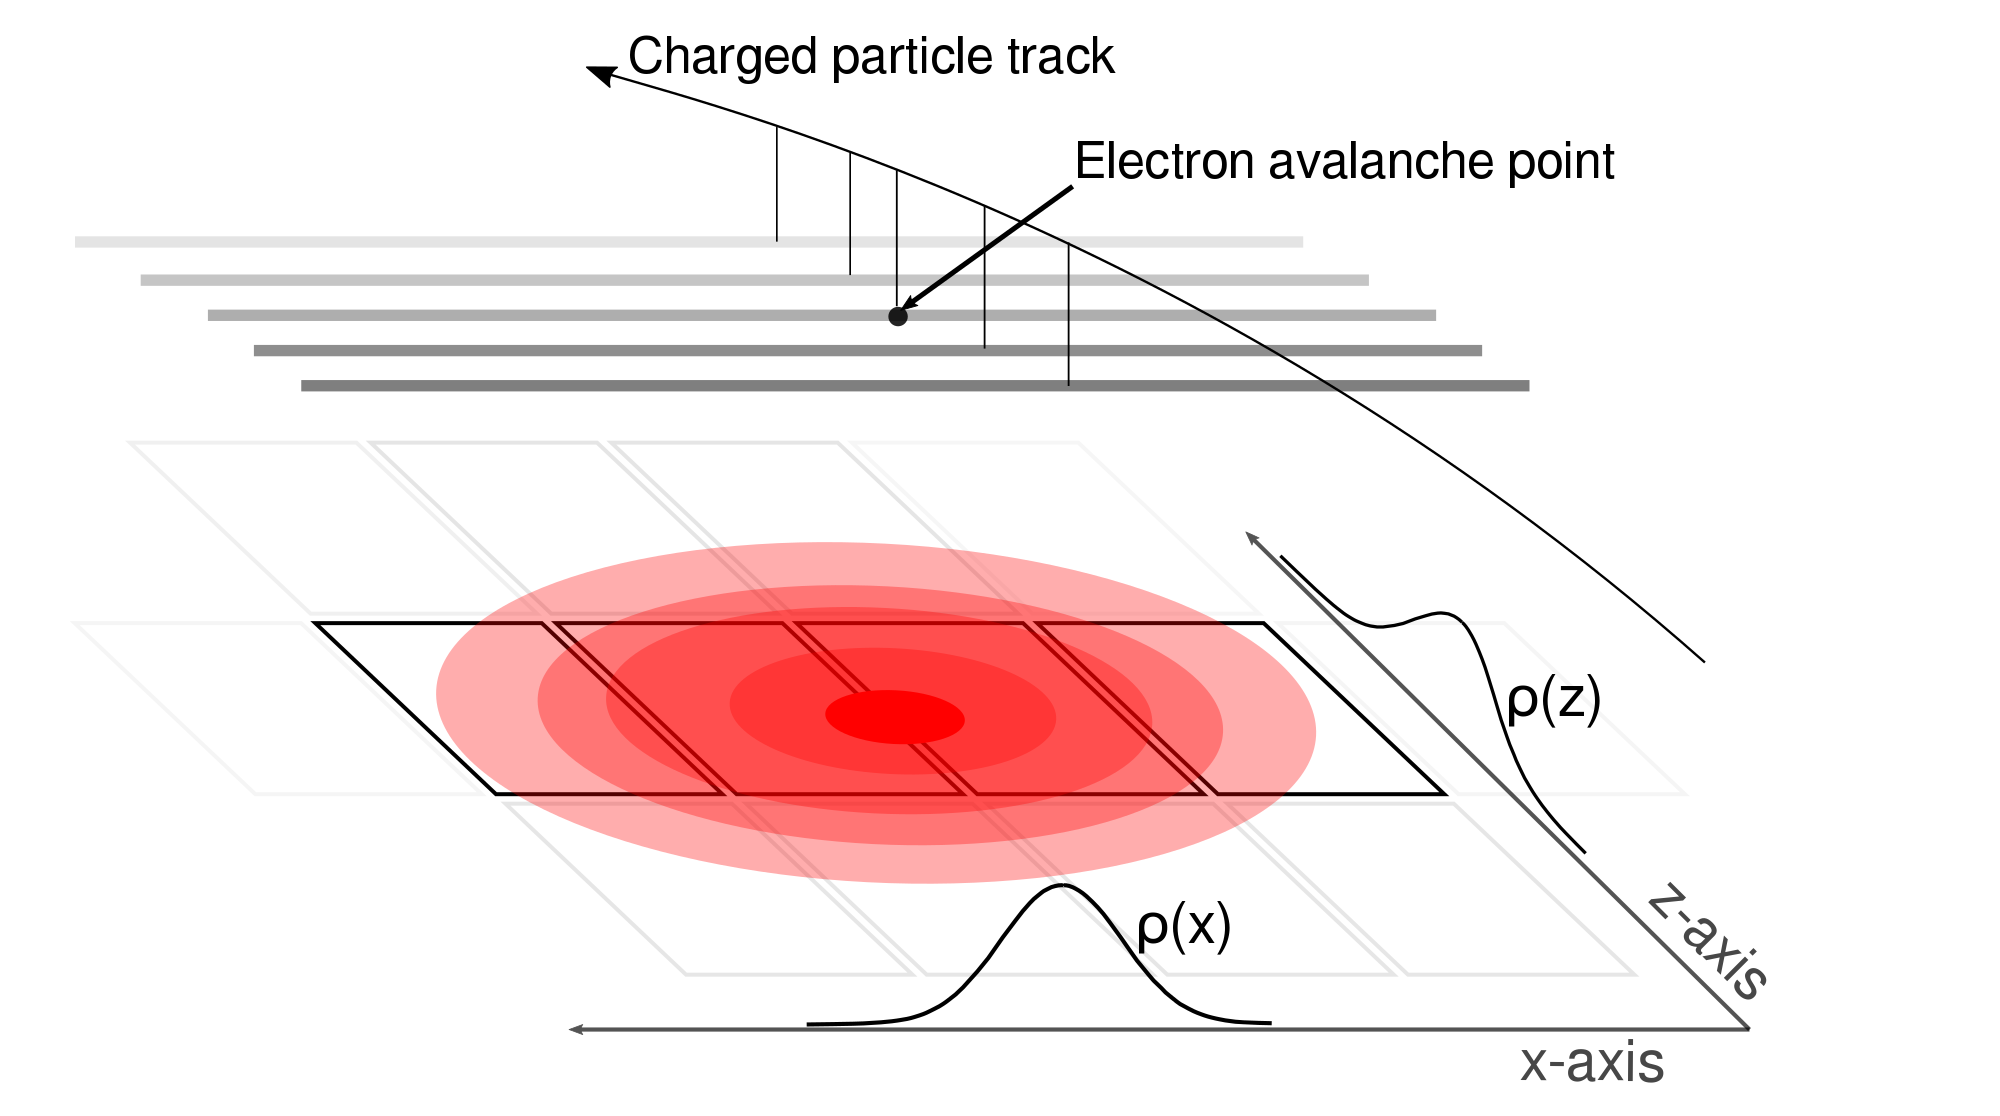
\includegraphics[width=\linewidth]{padsat_Large}
\caption{A cartoon illustration of the charge distribution resulting from an electron avalanche on one wire and the projections of the distribution onto the two axis $\rho(x)$ onto the x-axis and $\rho(z)$ onto the z-axis. The orientation of the wire planes is flipped upside down to display the perspective better.}
\label{fig:2DPRF}
\end{figure}

Gatti \cite{gatti} derived a semi-empirical formula for the charge distribution in a simple multi-wire TPC given as, 
\begin{equation}\label{eq:gatti}
\begin{split}
PRF_{\mathrm{Gatti}}(\lambda)
& = \frac{K_{1}}{K_{2}\sqrt{K_{3}}}\bigl[\arctan(\sqrt{K_{3}}\tanh\bigl[K_{2}\bigl(\frac{\lambda}{h}+\frac{w}{2h}\bigr)\bigr]) \\
& - \arctan(\sqrt{K_{3}}\tanh\bigl[K_{2}\bigl(\frac{\lambda}{h}-\frac{w}{2h}\bigr)\bigr])\bigr] \\
\end{split}
\end{equation}

where $w$ is the width of the pad, $h$ is the distance of the anode plane to the pad plane, and $\lambda$ is the distance of the pad center to the avalanche point. It is a single parameter equation where the two parameters $K_1 = \frac{K_{2}\sqrt{K_3}}{4 \arctan(\sqrt{K_3})}$ and $K_2 = \frac{\pi}{2}\left(1-\frac{\sqrt{K_{3}}}{2}\right)$ depend on the parameter $K_3$, which is a function of the ratio of the anode wire diameter to the distance of the anode wires to the pad plane. $K_3$ can be looked up in a graph in \cite{blumrol} and \cite{gatti}.


\begin{figure}[!htb]
\begin{overpic}[width=\linewidth]{fig5.pdf}
\put(61,55){\contour{white}{ PRF${}_{\mathrm{Gaus}}(\lambda)$ eq. \ref{eq:gaus}  }}
\put(61,49){\contour{white}{ PRF${}_{\mathrm{Gatti}}(\lambda)$ eq. \ref{eq:gatti} }}
\end{overpic}
\caption{Experimental pad response function of many events for a crossing angle of $85^{\circ} < \theta \leq 90^{\circ}$.  }
\label{fig:expprf}
\end{figure}


Since we take the marginal distributions only along one layer or row of pads, correlations are introduced in the PRF from adjacent layers or rows which cause slight deviations from the expected Gatti distribution. Also, analytic PRFs only exist for classical multi-wire TPCs. For these reasons it is useful to experimentally measure the PRF and fit it with an empirical function, typically a Gaussian, to describe its behavior. The method for extracting the experimental PRF will be discussed latter, but by averaging over many events in the experimental data, the resulting PRF for the S$\pi$RIT TPC is shown in Figure~\ref{fig:expprf}. Here we see the deviations from the expected analytic Gatti distribution (black curve), whereas fitting with a two parameter Gaussian function (red curve) gives a better description of the  data, Eq.~\ref{eq:gaus}, with the two parameters being the normalization coefficient, $N_0$, width $\sigma$, and with a mean value assumed to be 0.

\begin{equation}\label{eq:prfgaus}
PRF_{\mathrm{Gaus}}(\lambda) = N_0 e^\frac{-\lambda^2}{2\sigma^2}
\end{equation}

While the differences between the Gaussian distribution and the Gatti distribution are small for this TPC geometry, we use the Gaussian distribution because of its superior reproduction of the tails of the pad response function.   



\begin{comment}
\subsection{Considerations when constructing a TPC}
Several considerations went into the construction of the S$\pi$RI TPC which I wish to summarize and document here. All materials and glues of the TPC were selected as low out-gassing materials. Several materials (that are common place in nuclear labs), such as vacuum grease, Viton o-rings, all out-gas organic chemicals into the counter gas which damage the TPC by permanently lowering the gain over time. The organic molecules responsible are difficult to identify exactly, but lists of good and bad materials are well known in the literature from experiments. If a material we wished to used was not on these lists we placed the material in a clean chamber with the counter gas and flowed this counter gas through a small proportional counter making sure the gain did not drop at high collection rates when exposed to a high rate alpha Americium source. 

Sparking
Two volumes of gas. 
\end{comment}


\section{Radio Isotope Beam Factory (RIBF) Facility }
%Cyclotron facility overview.
%Samurai line overview.
%Beam line element overview.
%Big rips beam PID. reference 
The primary and secondary beams were produced at the Radioactive Isotope Beam Factory (RIFB) facility at RIKEN, in Wako-shi, Japan. The RIBF facility starts with two primary beam types, ${}^{132}$Xe and ${}^{238}$U, which are produced by an ion-source and accelerated to progressively higher kinetic energies by 1 linear accelerator (RILAC), and 4 different cyclotrons (RRC, fRC, IRC, and SRC), until they reach a beam energy of \SI{345}{\MeVA}. Figure~\ref{fig:samuraiBeamLine} shows the later stages of the cyclotrons and the following beam lines to which these beams can be sent. For this dissertation, the beam went through the BigRIPS spectrometer, where the specific rare isotope beams of interest were produced and on to the SAMURAI dipole where the  \spirit TPC was placed. The red box indicates the location of the experimental setup in Figure~\ref{fig:samuraiBeamLine} .


\begin{figure}[!htb]
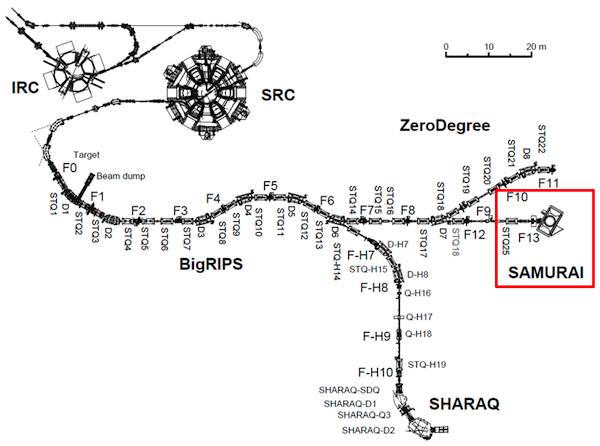
\includegraphics[width=\linewidth]{SAMURAI-beamline.png}
\caption{Overview of the RIBF, BigRIPS, and SAMURAI beamline.}
\label{fig:samuraiBeamLine}
\end{figure}

After the SCR, the primary beams impinge on a rotating \SI{3}{\milli\metre} Be target which fragments the beam into many different species. These fragments are then separated by the BigRIPS spectrometer which is tuned to the particular secondary fragment of interest. This is accomplished through several dipole magnets, slits, and wedge degraders. The resulting secondary beam is not pure and the purity depends on the capability of BigRIPS to deliver the secondary beam of choice and the primary beam used. The BigRIPS separator had many scintillators for timing, an ion chamber for Z identification and beam tracking elements used to determine the magnetic rigidity of the beam. Information from these detectors allow  allowed  identification  of the mass, charge and momentum of each isotope in the secondary beam. This information was determined beam particle by beam particle and recorded along with the TPC data on each event. With this information, it was possible to select with precision the reactions to be included in any subsequent data analysis.  

In the experimental campaign,   several beams were utilized that have  different intensities and purities. Table~\ref{tb:beams} summarizes the average qualities of the 4 secondary beams that were used in our experimental campaign. Most beams were delivered with an intensity of \SI{10}{\kilo\hertz}.

 \begin{table*}\centering
\ra{1.3}
\begin{tabular}{@{}ccccc@{}}\toprule 
 Primary Beam & Secondary Beam & Energy at mid target \si{\MeVA} & Intensity \si{\kilo\hertz} & Purity (\%) \\ [0.5ex] 
 \midrule
 ${}^{238}$U   & ${}^{132}$Sn   &  269.2  &  9.5  &  54   \\
 ${}^{238}$U   & ${}^{124}$Sn   &  270.3  &  9.1  &  10  \\
 ${}^{124}$Xe  & ${}^{112}$Sn   &  270.4  &  7.6  &  48  \\
 ${}^{124}$Xe  & ${}^{108}$Sn   &  269.3  &  7.5  &  52   \\
 \bottomrule
\end{tabular}
\caption{Primary and secondary beam properties produced in the \spirit TPC experimental campaigns. }
\label{tb:beams}
\end{table*}



\section{Experimental Setup}

The \spirit TPC was designed to fit exactly into the dipole gap of the  dipole magnet at the end of the BigRIPS beam line. Figure~\ref{fig:experiment} shows a drawing of the \spirit TPC inside of the SAMURAI magnet chamber which was rotated to the $\ang{0}$ configuration. Typically the SAMURAI (Superconducting Analyzer for Multi-particles from Radioisotope beams) dipole magnet is operated under vacuum as a large-acceptance multi-particle spectrometer for radioactive-beam experiments. This magnet can reach magnetic fields up to \SI{3}{\tesla} at the center of the pole gap and was operated at \SI{0.5}{\tesla} for these sets of experiments. The space between the magnetic pole faces is further complicated by large bolts which protrude from the pole faces. These bolts secure the vacuum chamber to the magnet which is not practically removable; though the inside of the magnet was not operated under vacuum. This required an extensive rail system and support frame to slowly slide in the TPC over the bolts, finally raising the TPC several \si{\centi\metre} to the final height. 

\begin{figure}
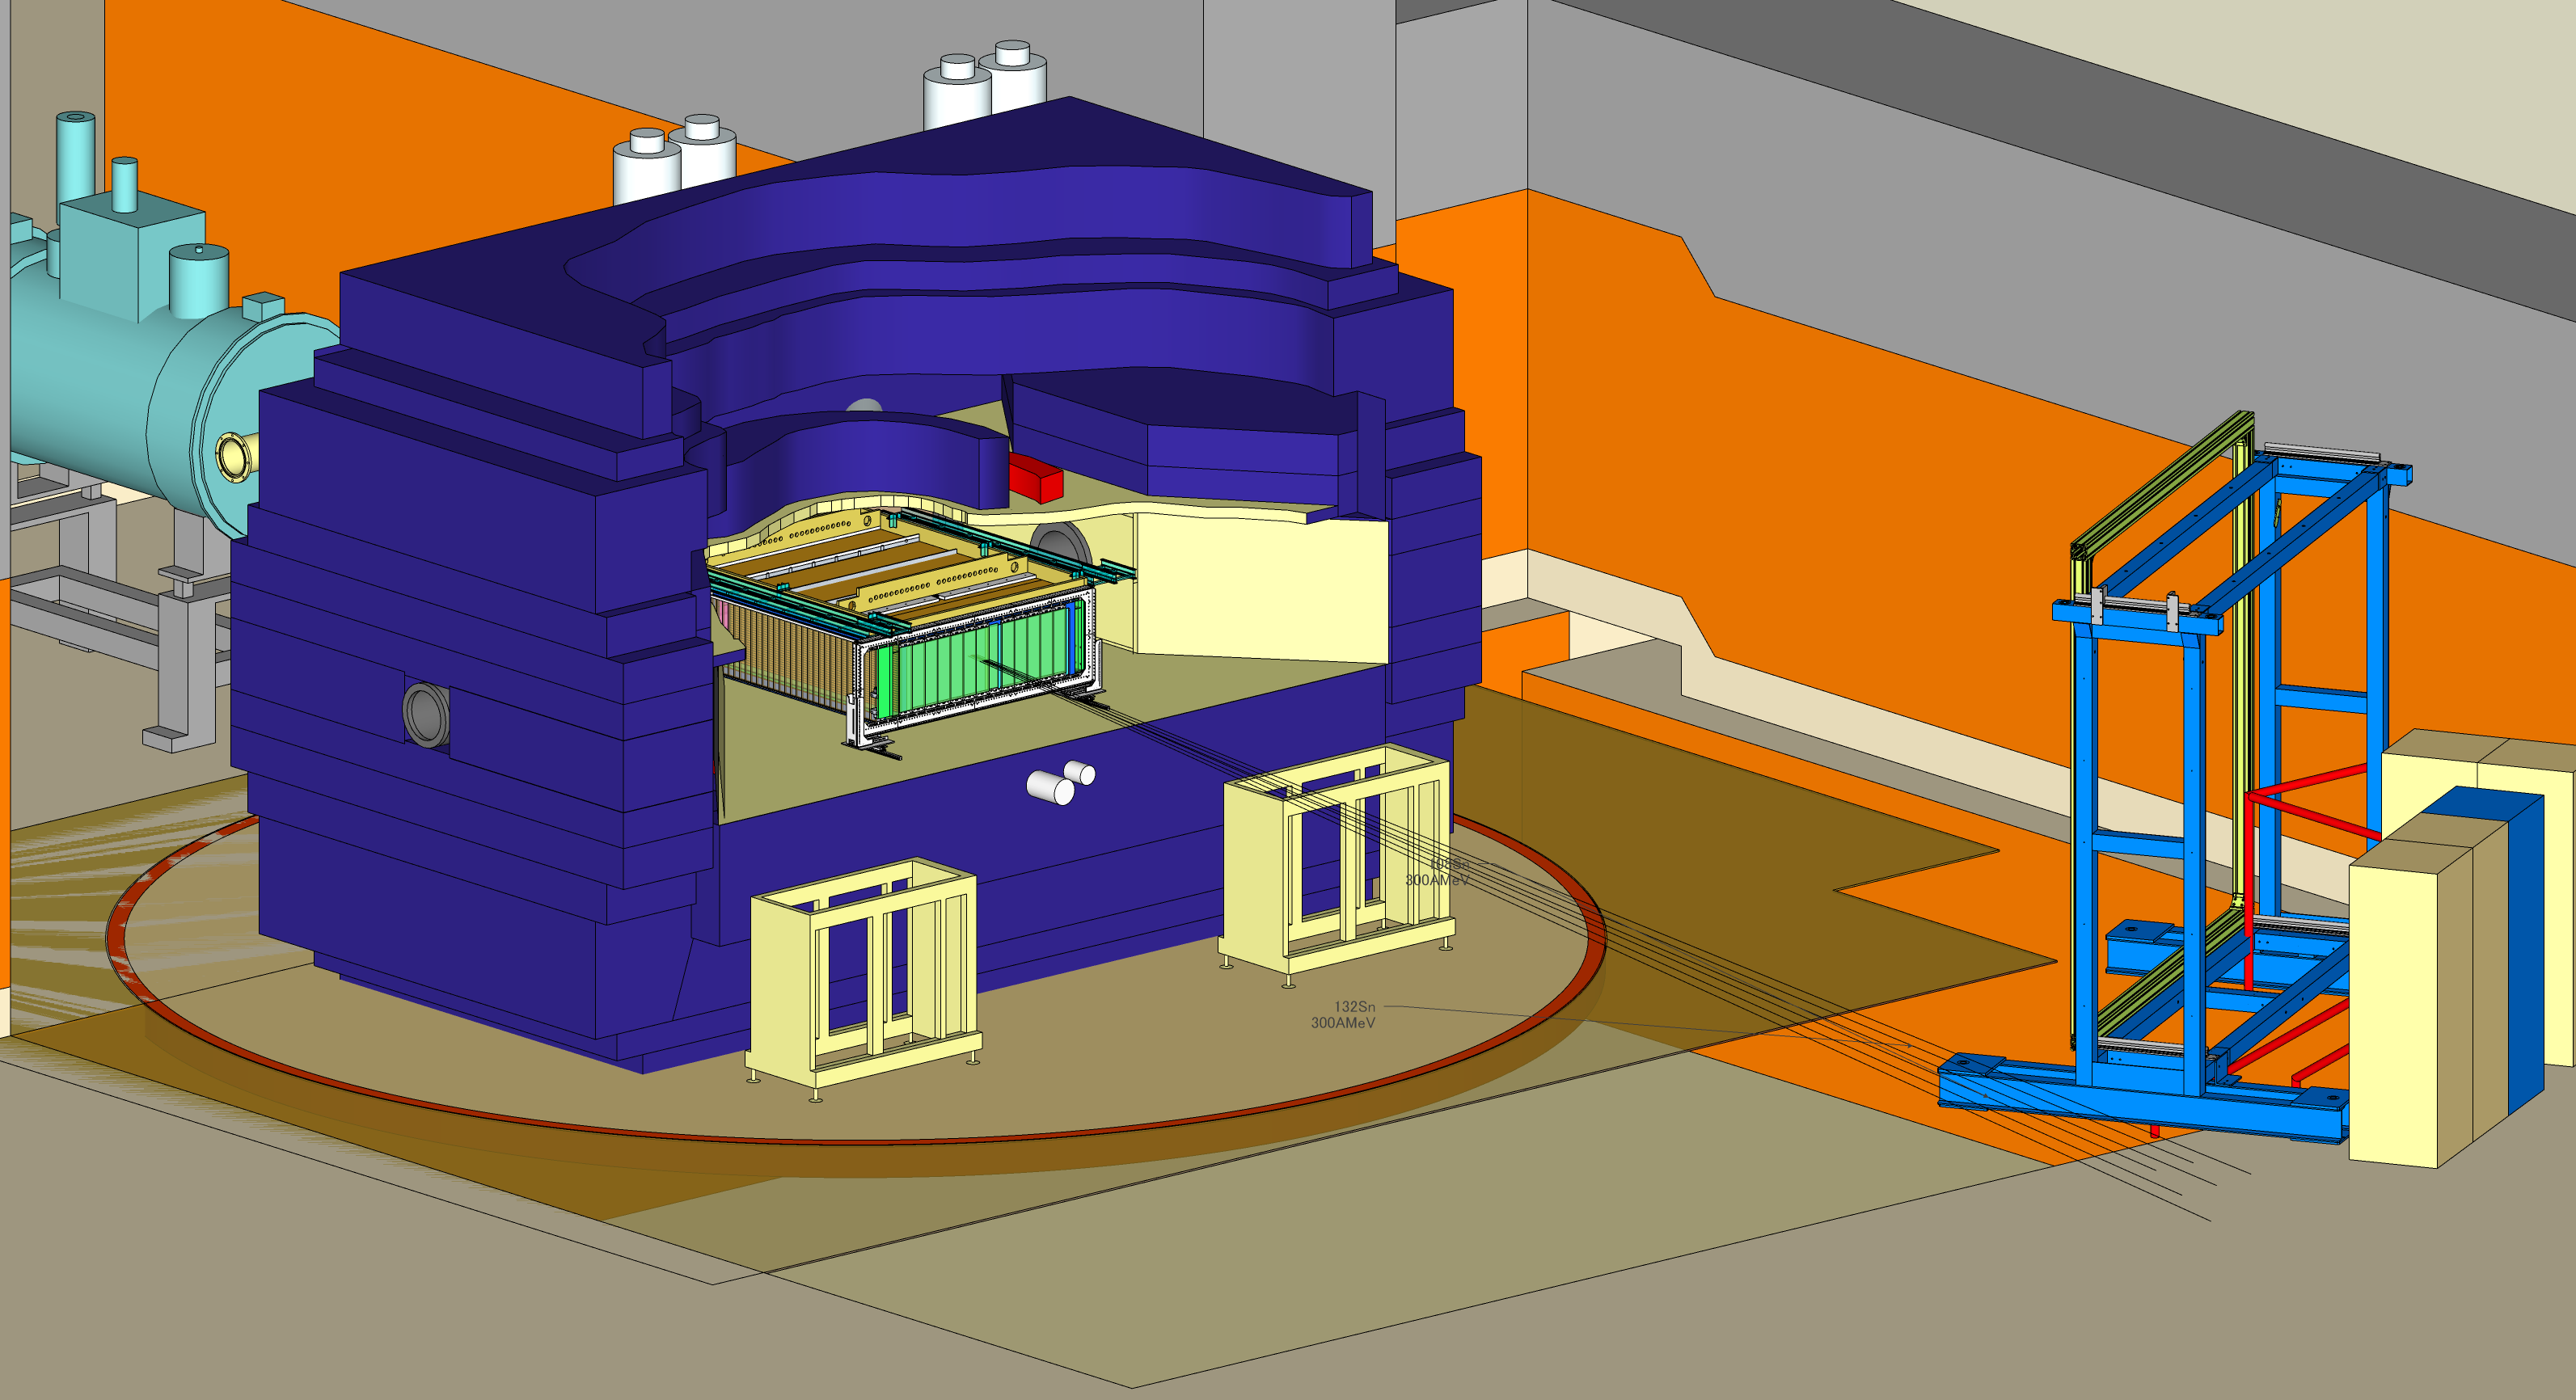
\includegraphics[width=\textwidth]{perspective.png}
\caption{Drawing of the experimental setup with the TPC inside of the SAMURAI magnet at $\ang{0}$ configuration.}
\label{fig:experiment}
\end{figure}

The height of the TPC was roughly aligned with a self-leveling laser system to match the center of target with the center of the beam line. Once the TPC was adjusted to the final location, the position of the TPC was measured in fine detail with a the VStars-N photogrametry system \cite{vstars}. Small highly reflective targets were placed all over the TPC both inside and out and pictures were taken with a calibrated lens and camera system. Using the commercial software provided the set of different camera perspectives was reconstructed into a 3-dimensional point cloud of all the targets. Since the magnet was also measured with the same system after installation, we can match the two systems to get the absolute position of the TPC, and its internal components, relative to the magnet frame. The position resolution of this type of system was estimated to be around \SI{200}{\micro\metre} for each coordinate, which is much more precise than needed or Show data.

The origin of the \spirit TPC was defined to be at the center of the TPC pad plane in the x-direction and at the edge of the last upstream pad. The center of the magnet is defined as the center of the magnet in x and z-directions and the middle of the dipole gap in the y-direction. The origin of the \spirit TPC in the magnet frame is (1.794,205.502,-580.526) for x,y,z-coordinates in units of \si{\milli\metre}. The error in each coordinate estimated to be (.2,.1,.4) \si{\milli\metre} respectively. 

%Maybe put a position table summary here of the TPC position and definition of the coordinates system in the TPC frame and the Magnet frame

\section{Beam Drift Chambers (BDC)}
\label{sec:bdc}

There were two beam drift chambers (BDC) located along the beam pipe upstream of the magnet and after the last focusing quadropole magnet. These beam drift chambers contained two sets of parallel plate avalanche counters (PPAC) which could get the (x,y) coordinates of the beam. Since they were places approximately \SI{1}{\metre} apart, we were able to track the direction of the beam in the beam line using a linear extrapolation. The resolution of the initial angle the beam enters the SAMURAI dipole was estimated to be \SI{0.64}{\milli\radian} and \SI{0.24}{\milli\radian} for the two angles defining the beam vector \cite{jon}. The initial angle, energy, and charge of the beam is then propagated through the magnetic field map until the angle on target is found. The angle on target though small will be important later for transforming back into the center of mass system as will be seen in Section~\ref{sec:beamangle} and Section~\ref{sec:pionSpectra}.


\section{Ancillary Detectors }
Several ancillary detectors were placed inside and outside of the \spirit TPC to facilitate in making the trigger for the experiment. The ability of ancillary detectors to work effectively when placed outside the TPC  was one of the more important considerations we made when designing the TPC. A brief description of each ancillary detector system is given here with particular focus on how the experimental trigger was made. 


\subsection{Kyoto Multiplicity Trigger}
\label{sec:kyoto}
%kyoto array sets multiplicity trigger
%scintillator bars
 The Kyoto Multiplicity Array, shown in Figure~\ref{fig:aux}, consists of two arrays of plastic scintillating bars on each side of the TPC, each consisting of 30 bars. The entire TPC structure was designed so that light charged particles could pass through the field cage and side walls of the TPC enclosure without excessive energy loss and scattering. This allowed the number of tracks passing through the sides of the TPC could be measured by in an external array. In heavy ion collisions the more central a nuclear collision is, the more nucleons participate in the collision, resulting in a higher observed track multiplicity. It is this correlation between the number of tracks and centrality of the collision that makes the number of hits in the Kyoto Array sensitive to the centrality of events. It is more likely that in very central collisions more tracks are going to the large angles and measured by the Kyoto array. In the experiment the trigger selection criteria was $n_{Kyoto} > 4$, where $n_{Kyoto}$ is the total number of tracks measured by both arrays. The Kyoto array proved to be a good trigger that suppressed peripheral collisions; this will be discussed in later sections. 

\begin{figure}[!htb]
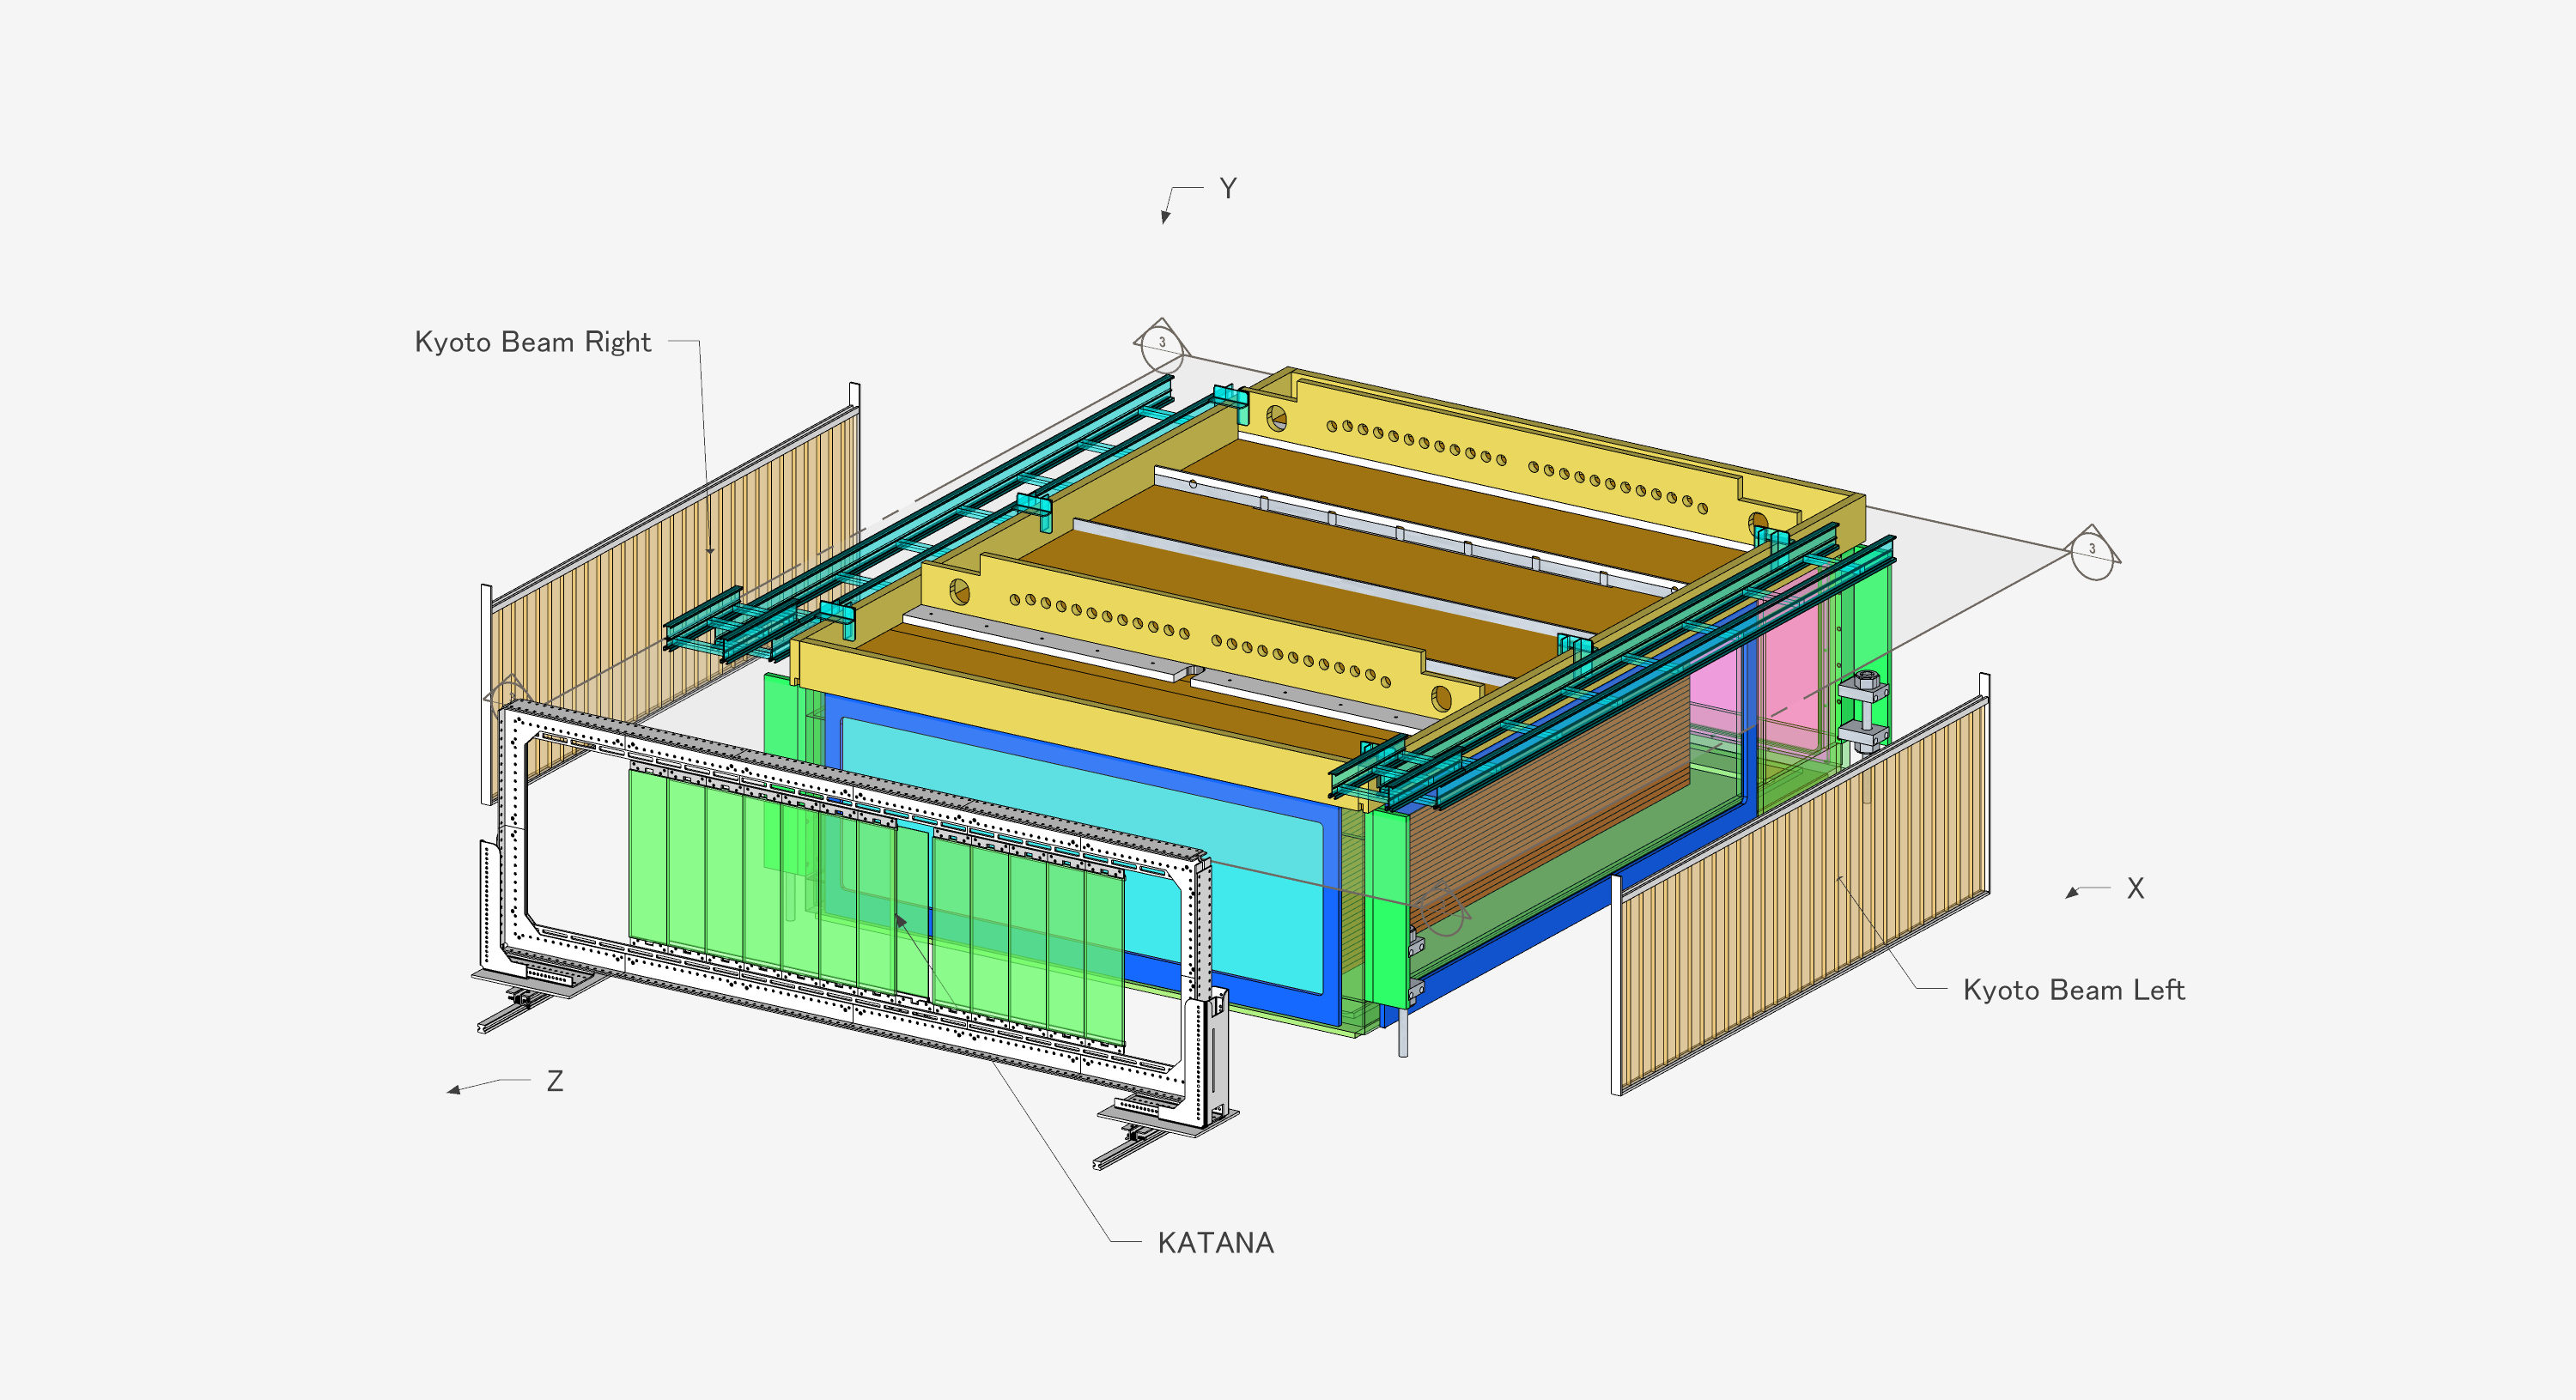
\includegraphics[width=\textwidth]{TPCAux.png}
\caption{Exploded views of Kyoto and KATANA arrays.The Kyoto array elements are in tan and are located on the left an right side of the TPC. When they are in place, they are nested against the thin aluminum side windows of the TPC. The KATANA array is in green and is located adjacent to the downstream window of the TPC.}
\label{fig:aux}
\end{figure}


\subsection{Krakow KATANA Veto and Multiplicity Array}
%beam veto
%beam trigger optional
 Figure~\ref{fig:aux} also shows the Krakow KATANA array, which consists of 12 plastic scintillating bars mounted adjacent to the downstream wall of the TPC enclosure. Three of the 12 bars 1 mm in thickness and operated as a beam veto in the event the beam did not make a nuclear collision with the target; this occurred approximately 99\% of the time. The 9 other bars were 1 cm in thickness and provided additional information about the light particle multiplicity array similar to the Kyoto array. We found that a large number of events involved peripheral collisions and active target events in which the beam interactions with the counter gas. Active target events contributed to a large multiplicity in the KATANA but not to the Kyoto array. So multiplicity $M_{Kyoto} > 4$ in the Kyoto array combined with a veto on events with a forward going projectile remnant with Z>20 provided the most effective suppression of peripheral collisions and active target events. Thus the KATANA array was used in primarily the beam veto mode. This was accomplished by positioning the array so that the expected position of the beam exiting the TPC would be centered on the three thin paddles. The threshold of the veto paddles were set so that the charge of a particle passing through, $Z$, would veto any event that satisfied $Z > 20$, where the charge of the Sn beam is $Z=50$. 


\subsection{Active Veto Array}
The beam was tuned by two sets of quadrupole  magnets, STQ 1 and STQ2 (as seen in Figure~\ref{fig:samuraiBeamLine}), so that the beam spot was focused on the TPC target location. Because of the inherent angular dispersion of the beam there still were incoming beam events which significantly deviated from the target location. These could be suppressed in the analyses by a gate on the reaction vertex; however, there remained a concern about the dead time such target frame events would contribute and how this would limit the amount of good data we could obtain.  To veto these type of events an active veto array was set at the entrance of the TPC consisting of four small scintillating bars arranged to be slightly larger than the target size. The threshold was set so that any beam particle which passed through any of the bars it would send a trigger signal to not trigger the system since the beam path would not be on target but on some other material inside the TPC. Minimizing these active veto rates also proved to be useful when tuning the beam so as to be centered on the target.


\section{Data Acquisition (DAQ) }
The Data AcQuisition (DAQ) consisted of three different systems. The RIBFDAQ system served as the master DAQ for the BigRIPS beam identification DAQ, the TPC DAQ, the NeuLAND neutron wall DAQ, and the Kyoto Array DAQ systems. The TPC DAQ was handled by the NARVAL framework to readout the GET electronics for the \spirit TPC. A General Trigger Operator (GTO) trigger was supplied to each DAQ synchronizing the subsystems. 

\section{Trigger Condition}
Signals from all of the auxiliary detectors were combined into several logic combinations to form a trigger logic for triggering the data acquisition  (DAQ) to record data. An upstream scintillating bar formed the start counter signal, triggering on any beam coming down the beam line. The active veto will trigger for any beam that is off the target location. The KATANA veto produced a signal if the beam passed through the TPC un-reacted, causing no nuclear collision; this produces a veto signal with a width of \SI{4}{\micro\second} which is the approximate time it takes for the beam to drift and clear the field cage volume. The Kyoto multiplicity trigger produces a signal when the total number of tracks passing through both Kyoto arrays are greater than 4. 


\begin{figure}[!htb]
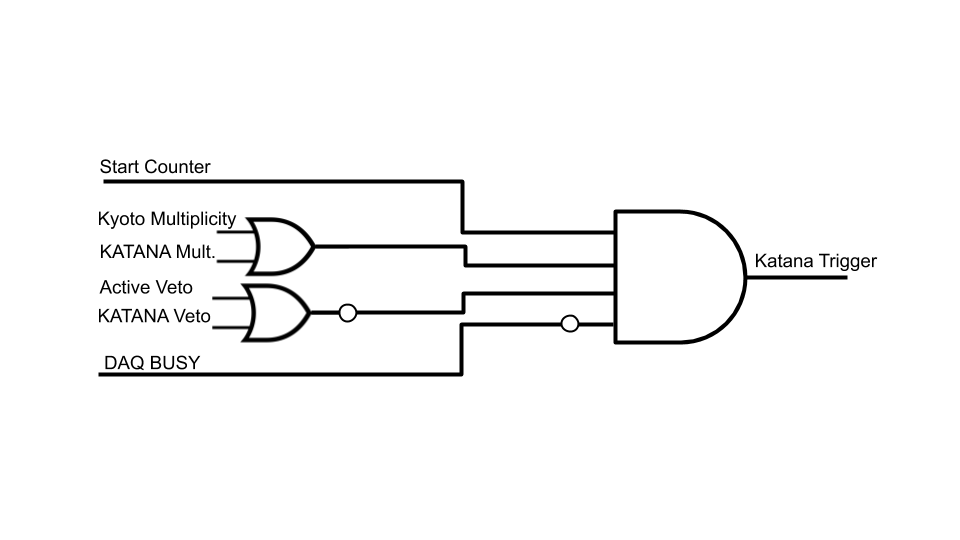
\includegraphics[width=\linewidth]{KatanaLogic.png}
\caption{KATANA trigger box logic.}
\label{fig:katanaLogic}
\end{figure}

\begin{figure}[!htb]
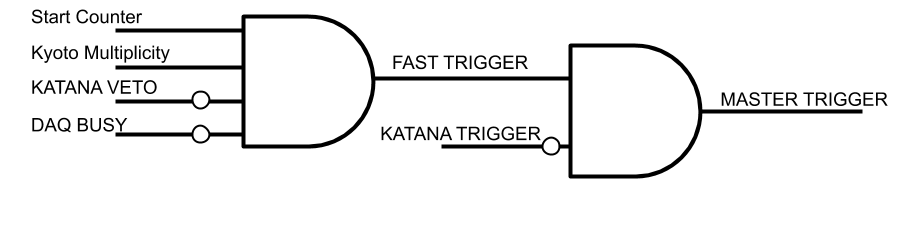
\includegraphics[width=\linewidth]{TriggerLogic.png} 
\caption{Master trigger logic.}
\label{fig:trigLogic} 
\end{figure}

\begin{figure}[!htb]%
    \centering
    \subfloat[${}^{124}$Xe primary beam trigger.]{{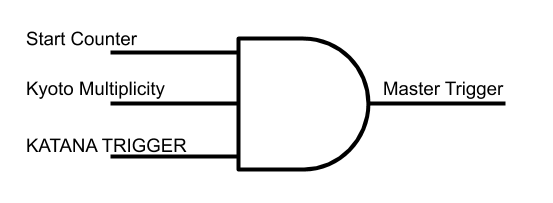
\includegraphics[width=.45\textwidth,valign=t]{DataTrigger1.png} \label{fig:dataTrigger1}}}%
    \qquad
    \subfloat[${}^{238}$U primary beam trigger.]{{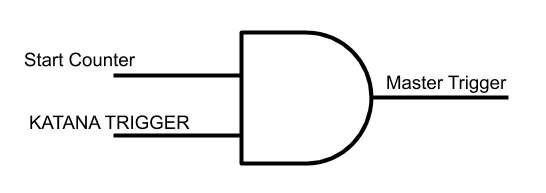
\includegraphics[width=.45\textwidth,valign=t]{DataTrigger2.png} \label{fig:dataTrigger2}}}%
	\caption{Master triggers in each primary beam setting.}    
	\label{fig:datatrigger}
\end{figure}

There were several special trigger considerations incorporated into the trigger for the TPC. We required that the gating grid be opened quickly to not lose electrons from portions of the tracks that pass close to the gating grid. If the DAQ was not busy, we therefore generated a trigger once we had a start detector signal, a Kyoto multiplicity >4 signal, and neither a Katana Veto signal nor an active target signal. This was referred to as the Fast Trigger, and it triggered the opening of the gating grid, which took about 350 ns. Following the initial trigger, we had the possibility of a fast clear signal that could be initiated by a later beam particle traversing the TPC. If the last beam particle came within 4 us after the fast trigger, electrons from this beam particle could pass through the gating grid. Such data would be useless, so we closed the gating grid and stopped the data acquisition with a fast clear signal. Additional fast clears could also initiated if the Katana trigger box did not generate a trigger. Figure~\ref{fig:trigLogic} shows the logic of both of these triggers.

The Katana trigger box took some time to completely master, it did not take on the major trigger responsiblities at first. In later runs, most of the trigger functions were performed the in Katana trigger box. The master trigger for the DAQ was different for each primary beam as the experiment got progressively better. During the ${}^{124}$Xe primary beam, the KATANA trigger box was an input into the trigger logic, where as in the ${}^{238}$U primary beam, the KATANA trigger box functioned as the trigger logic utilizing the internal trigger electronics. In either case the differences in the trigger logic were very minor and they both behaved practically the same except for minor details on the gating-grid trigger \cite{jon}. Figure~\ref{fig:katanaLogic} summarizes the KATANA trigger box logic. 

Figure~\ref{fig:dataTrigger1} summarizes the ${}^{132}$Xe primary beam, where the condition to produce a true KATANA trigger output was there must be a Start Counter, KATANA multiplicity, no Veto, and no DAQ busy signal. The KATANA trigger, Kyoto Multiplicity, and Start Counter together triggered the DAQ. 

 Figure~\ref{fig:dataTrigger2} summarizes the ${}^{132}$Xe primary beam, where the condition to produce a true KATANA trigger output was there must be a Start Counter, Kyoto or KATANA multiplicity, no Veto, and no DAQ busy signal. Here the KATANA trigger and the SC SUM together triggered the DAQ. 
 
 %I don't think this is true.
 
 It is worth mentioning how the busy signals for the experiment were handled. The DAQ system itself produces a busy signal which was combined in an OR with the busy signals from either the opening or closing the gating grid. When opening the gating grid, it is assumed the full volume of the TPC will be read out, therefore  a \SI{11}{\micro\second} gate busy signal is produced; which is slightly more than the time it takes for all the electrons to drift in the field cage. In the case were the gating grid should be closed, either due to the fast clear circuit or the end of the TPC measurement, a \SI{5}{\micro\second} busy signal is produced to allow for the gating grid to settle to a steady state closed configuration, and to clear the drift volume of any residual electrons from the beam. Both of these gates are included with the DAQ in an OR configuration which makes the overall busy signal. 
 


\section{Collision Data Taken}

Figure~\ref{fig:data} shows the example pad plane readout of the TPC from a central nuclear collision of Sn + Sn. Here we can see several tracks resulting from a single vertex location which is near the target region. The color values represent the max ADC observed in a given pad. The large amount of saturation that occurs in the electronics which is represented by the brightest yellow value. Also the lower voltage anode sections described in Section~\ref{sec:wireplanes} are denoted by red arrows. The pads directly over these wire planes have an effective gain reduction due to the lower anode voltage on the wires. Tracks with a high enough energy loss continue through these sections, but tracks with low energy loss values do not deposit enough energy and disappear, only to reappear in the higher gain section in between. 

\begin{figure}[!htb]
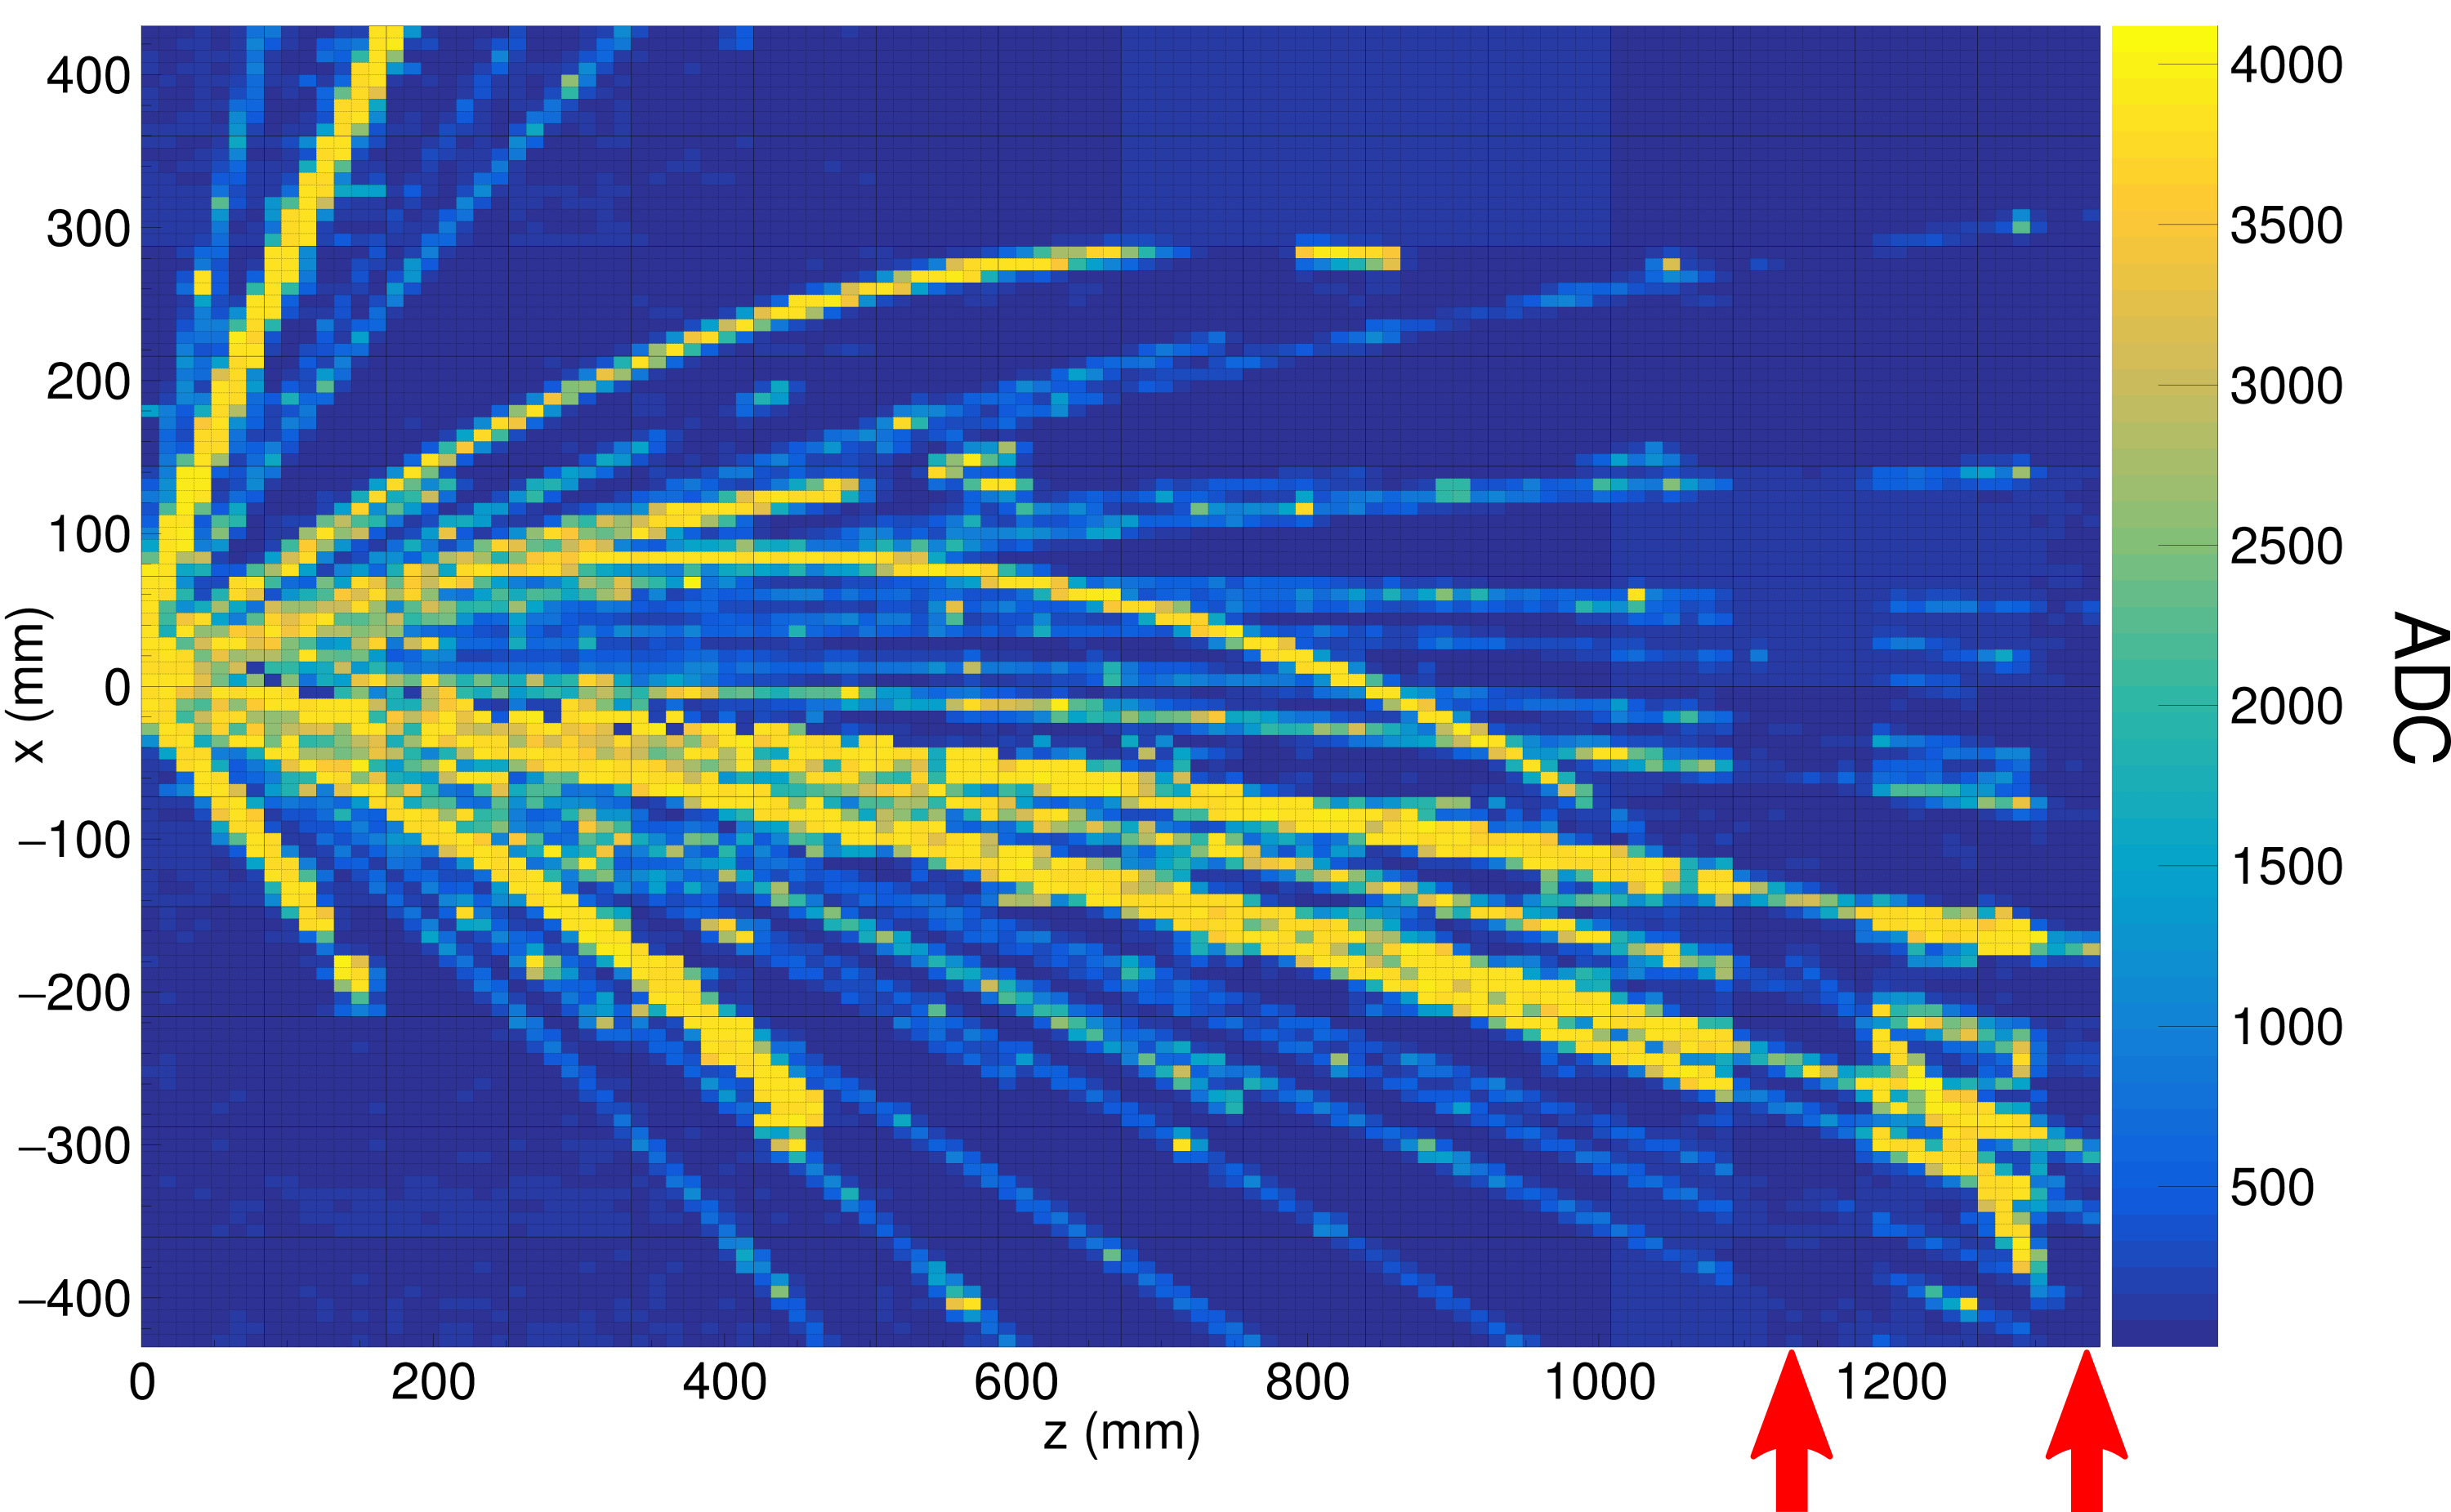
\includegraphics[width=\linewidth]{data.png}
\caption{Pad plane projection for a collision event in the TPC. Highlighted by red arrows are two regions of anode wires which had a reduced voltage of 1214 V. The voltage of the rest of the TPC anode wires are 1460 V. The reduction in voltage reduces the gain by a factor of about 10. }
\label{fig:data}
\end{figure}



Shown in Figure~\ref{fig:cocktail} is a typical cocktail event, where one particle enters the TPC volume at a time and parallel to the pad plane, representing an ideal case for momentum and $dE/dx$ determination; as it does not suffer from inefficiencies of high multiplicity events seen in the collision experimental data. The primary goal of this data set was to calibrate the TPC in both momentum and dE/dx as will be discussed in Section~\ref{sec:cocktail}. 

\begin{figure}[!htb]
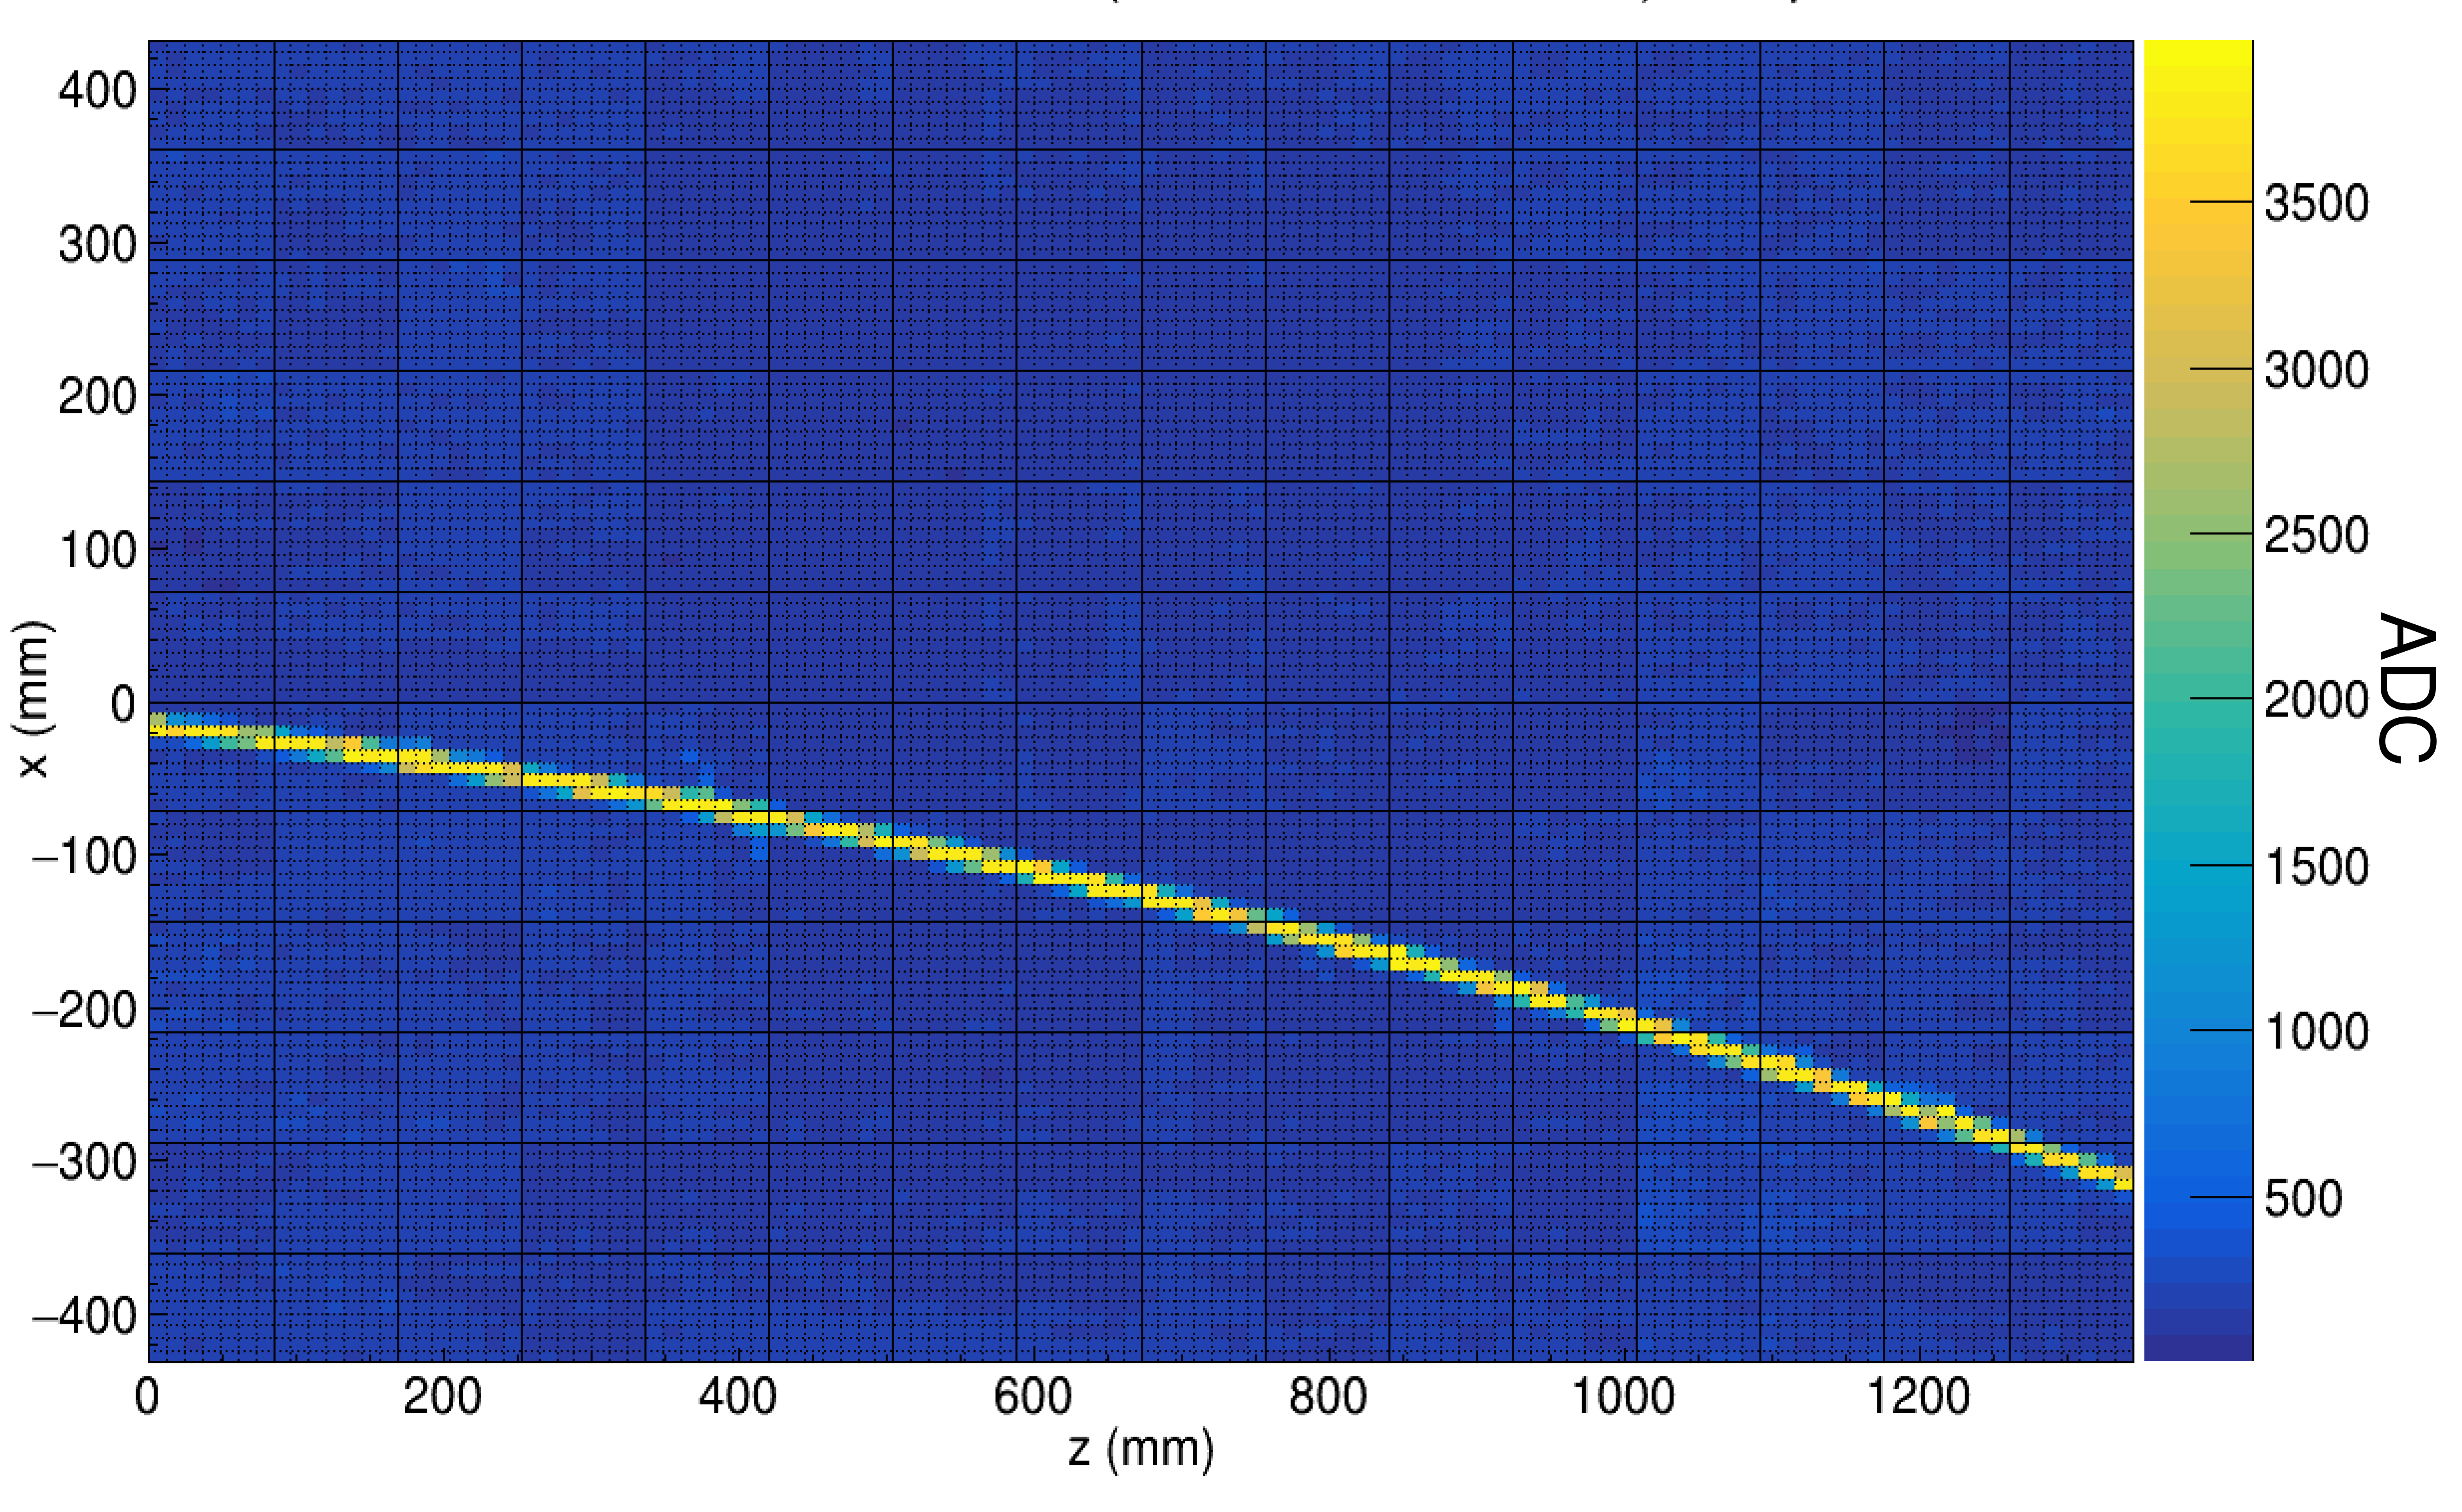
\includegraphics[width=\linewidth]{cocktail.png}
\caption{Pad plane projection for a cocktail event in the TPC.}
\label{fig:cocktail}
\end{figure}


